%% \documentclass[preprint,review,12pt]{elsarticle}
%% \documentclass[final,1p,times]{elsarticle}
%% \documentclass[final,1p,times,twocolumn]{elsarticle}
%% \documentclass[final,3p,times]{elsarticle}
%% \documentclass[final,3p,times,twocolumn]{elsarticle}
%% \documentclass[final,5p,times]{elsarticle}
%% \documentclass[final,5p,times,twocolumn]{elsarticle}
%% \usepackage{graphics}
%% or use the graphicx package for more complicated commands
%% \usepackage{graphicx}
%% or use the epsfig package if you prefer to use the old commands
%\usepackage{epsfig}
\documentclass[preprint,12pt,3p]{elsarticle}
\usepackage{amssymb}
\usepackage{natbib,hyperref}
\usepackage{paralist}
\usepackage{color}
\usepackage{amssymb}
\usepackage{graphicx}
\usepackage{enumerate}
\usepackage{multirow}
\usepackage{multicol}
\usepackage{booktabs}
\usepackage{mathtools}
\usepackage[bottom]{footmisc}
\usepackage{libertine}
\usepackage{enumitem}
\usepackage[T1]{fontenc}
\usepackage[svgnames]{xcolor}
\usepackage[utf8]{inputenc}
\usepackage{cleveref}
\usepackage{float}
\usepackage{caption}
\usepackage{wrapfig}
\usepackage{subfig}
\usepackage{tikz}
\usepackage{longtable}
\usetikzlibrary{shapes, arrows,bending}
\usepackage{relsize}
\usetikzlibrary{positioning,calc, shapes,arrows}
\captionsetup[figure]{font=footnotesize}
\usepackage{setspace}
\usepackage[pagewise]{lineno}
\usepackage{tikz, tikz-qtree}
\usepackage{xcolor}
\usetikzlibrary{arrows, decorations.markings, calc, fadings, decorations.pathreplacing, patterns, decorations.pathmorphing, shapes.misc,positioning}
\usepackage{pgffor}
\usepackage{wasysym}
\setlist[itemize, 1]{label =\raisebox{-0.3\height}{\scalebox{2}{\textbullet}}}
\setlist[itemize, 2]{label =\raisebox{-0.3\height}{\scalebox{2}{\textbullet}}}
\tikzstyle{vecArrow} = [thick, decoration={markings,mark=at position 0 with {\arrowreversed[scale=2,semithick, DimGrey]{triangle 60};},
mark=at position 1 with {\arrow[scale=2,semithick, DimGrey]{triangle 60}}},
   double distance=1.4pt,shorten <= 5.5pt, shorten >= 5.5pt,
   preaction = {decorate},
   postaction = {draw,line width=5pt, DimGrey,shorten <= 5.5pt,shorten >= 4.5pt}]
   
 \tikzstyle{vecArrow1} = [thick, decoration={markings,mark=at position
   1 with {\arrow[scale=2, semithick, DimGrey]{triangle 60}}},
   double distance=1.4pt, shorten >= 5.5pt,
   preaction = {decorate},
   postaction = {draw,line width=5pt, DimGray,shorten >= 5.5pt}]

\urlstyle{same}



\journal{}

\begin{document}


\begin{frontmatter}


\title{Behavioural factors as a Driver/Barrier in the Energy Efficiency Renovation Decision-making Process: The Dutch homeowners} 



\author[label1]{Shima Ebrahimigharehbaghi\corref{cor1}}
\address[label1]{Delft University of Technology, Faculty of Architecture and the Built Environment, OTB, Julianalaan 134, 2628 BL, Delft, The Netherlands}
\ead{s.ebrahimigharehbaghi@tudelft.nl}


\author[label1]{Queena K. Qian}
\author[label1]{Henk J. Visscher}




\begin{abstract}

The Dutch climate change agreement incorporates ambitious targets that accomplishing them needs cooperation of all different sectors emitting green house emissions. The built environment has a share of 12.8\% in GHG emissions and can contribute as has happened in 2018 \citep{cbs2018}. The considerable share of owner-occupied sector, 70\%, shows the importance and potential offering of this sector in benefiting the built environment. This study aims to answer the questions of what behavioural factors influence the homeowners to make an energy efficiency renovation decisions. Mainly, the insight of behavioural economics are followed. The influencing factors from other behavioural studies are also covered to have a comprehensive overview of the factors.  The Woon enegy module 2019 is used to conduct the regression and statistical analysis for the Dutch owner-occupied sector, including the information of 2,878 homeowners. Approximately 46\% of householders perceive they consume less energy than what they actually consume. 




\end{abstract}

\begin{keyword}

Energy Efficiency \sep Renovations \sep behavioural factors  \sep Behavioural economic \sep Decision-making process \sep Owner-occupied sector

\end{keyword}

\end{frontmatter}



\pagebreak

\noindent
\textbf{Highlights}
\begin{itemize}
    \footnotesize
    \item [--] This study examined the behavioural factors influencing the renovation decision making process.
    \item[--] The expected and actual energy labels are different for the majority of householders. 
    \item[--] The energy label "A" and "C" has the highest correct expectations by householders.
    \item[--] 46\% of householders perceive consuming less energy than the actual consumption.
     \item[--] 67\% of householders perceive a higher energy label than the actual one. 
     
\end{itemize}

\section{Introduction}
\label{sec1}

The green house gas emission must be reduced by 49\% and 95\% by 2030 and 2050, respectively, written in the climate change agreement in the Netherlands. this target is too ambitious, since the GHG emissions should reduce twice in the next ten years compared to the last thirty years. The complementary targets such as 67\%  producing electricity and by renewable energy, and fully climate neutral electricity by these years are also aimed. Achieving these target seems suspicious according to the recent publication \citep{evert2019, Pbl2019}. Making the existing houses gas free is one of the major program. The current target is to make 30,000 to 50,000 houses per year gas free, but the final aim is to make 200,000 houses per year. This program would be effective when the houses have better insulation, higher efficiency boilers, and other sources of renewable energy are available for the housing stock \citep{rijk2019}. To support this program, government provides subsidies for the insulation, the heat pump or solar water heater for the houses \citep{rvo2019a, rvo2019b}. 


Housing stock has a high potential to contribute in reducing the energy consumption. Many research has identified the importance of occupant behaviour in explaining the energy consumption \citep{huebner2016, van2019actual}. These studies found almost 50\% of variations in energy consumption due to occupant characteristics and behaviours. In previous studies, it has been identified that there is a limited attention and interest in energy aspects of any type of renovations by householders, and the main motives of householders are cost-saving, increasing comfort, etc. 
The share of new built houses are minor in the last decade, almost 1 percent of the total housing stock \citep{cbs2020}. Therefore, the renovations of the existing dwellings seems to be a unique solution in achieving the energy efficiency target of the housing stock. The effectiveness of renovations are influenced by building and occupant characteristics \citep{van2019actual}. In the Netherlands, the owner-occupied sector has the highest share. For homeowners, the decision-making process should be entirely managed and conducted by the owners themselves. In which, it might be slower compared to the social housing sector, where a public authority can interfere and facilitate the implementation of energy efficiency renovations.  
\noindent

Occupant behaviours and characteristics are responsible for energy consumption in the housing stock \citep{huebner2016, guerra2010, steemers2009}. On the other hand, the majority of the houses are not new built and energy efficiency renovation seems the main approach in managing the energy consumption of the housing stock. Therefore, the aim is to study these behaviours and the impact on energy efficiency renovations in the Dutch owner-occupied sector. Several lines of research explain the logic of human behaviour including the behavioural economic, and psychologist. Additionally, engineering group of articles, we call them behavioural studies, are reviewed to cover a more comprehensive range of influencing factors in the analysis. The main emphasis of the current study is to understand the influencing factors, especially following the behavioural economist. This group of researcher aims to incorporate the psychological factors into the economic theories to explain behaviours that cannot be considered by the traditional economic theories. 

This paper is organised as follows. In section 2, the theories and backgrounds are presented classified into behavioural economics, psychological, and behavioural studies. In section 3, the research methodology is described, the database is explained, and statistical and logistic regression analysis are provided. The results of the analyses, discussion on these results, and conclusions are presented in sections 4, 5, and 6, respectively.

\section{Theories and Backgrounds}
\label{sec2}


\subsection{Theories: behavioural economist}

Compared to classical economist, the behavioural economist (BE) makes the distinction that people has cognitive limitations leading them to make irrational decisions. Decision making under risk and uncertainties is one of the factors that cause irrational decision. Also, many behavioural economist's theories are  inspired by Adam Smith theories, the theory of moral sentiments and the famous book of the wealth of nations. These influencing factors are for example the social norm, perceived fairness, and the social approval and status \citep{brekke2008}.


\subsubsection{Bounded rationality}

The unbounded rationality means that all the information is assumed to be accessible. However, in the theory of bounded rationality, the decision makers should be perceived as partially rational. Based on this proposition, \citep{simon1955, simon1979} developed a model by replacing the satisfaction instead of utility maximisation. Bounded rationality is not irrationality but optimisation under constraint \citep{gigerenzer2002}. The main characteristics of the agents with bounded rationality is that they often behave intuitively and that does not mean they reason inadequately. 

Three main categories of research explain the more realistic approach in studying the human behaviours. First, the heuristics (exploratory) approaches by people are not always the best available or rational options. The "availability heuristics" causes to many specific extra biases. Hindsight biases means that Events that has happened in the past are more probable to be imagined and expected by people than ones did not occur before \citep{camerer2004}. People might also have some biases due to the uncertainties surrounding them when they are predicting or evaluating the information or evidences. 

Second, a model that can explain the decision-making regarding biases different alternatives under risk or loss aversion in certain alternative. The prospect theory could explain the preferences to be determined by attitudes to gains and losses. Third, standard preferences theories combine a number of strong and testable assumptions. For example, preferences are "reference independent", constant relative to superficial variations, and etc. Different effects lead to violation of these theories. (1) "Framing effect is a cognitive bias and represents that the variations in the explanation of the outcomes affect the preferences of the people. This is in contrast with the essential aspect of rationality and rational decision-makers. (2) Anchoring effect also explains the violation of preferences to the standard theories regarding the preferences and refers to the willingness to be influenced by a pre-defined standard disregarding to its applicability. (3) Context effect means that ways in which preferences between choices are determined based on what other choices are available in contrast to  "independence of insignificant choices" (4) In standard theory, people are assumed to have invariant preferences  with respect to goods or endowments that they already have in their bundles. In contrast with this assumption, people seems to dislike much more loosing the current goods rather than having new goods which is called "Endowment effect" \footnote{For some specific circumstances such as resale this effect is not applicable. Also the "history of purchase effect" is important to how the preferences are invariant WRT to the bundles of good.}  \citep{klotz2010, kahneman2003, camerer2004}. 


\subsection{Theories: psychologist} 

This group of scientists explain the behaviour using theories such as Theory of Planned Behaviour (TPB) and Norm Activation Model (NAM). TPB assumes that the intention to take a behaviour passes the actual behaviour \citep{ajzen1991}. Regarding the acceptance of the sustainable energy technologies, two types of attitudes are related: (1) with regards to technologies, (2) with regards to a specific behaviour to the availability, e.g. purchasing or implementation of the sustainable energy technology, e.g. complaining about technologies (Fig \ref{fig:1}). NAM describes pro-social behaviour by stimulating the personal norms, i.e. moral obligations \citep{schwartz1977}. Regarding the sustainable energy technologies acceptance, awareness of the problems (e.g. environmental impacts) and outcome efficacy (contributing to effective solutions) are the determinants of personal norms. \citeauthor{huijts2012} propose perceived costs, risks and benefits as other factors influencing the personal norms (Fig \ref{fig:1}). 

\begin{figure}[H]
    \centering
    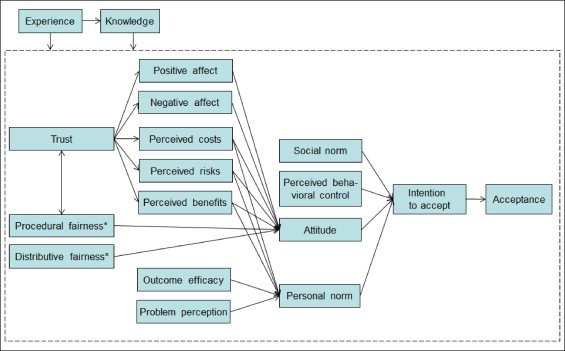
\includegraphics{PSYFR.jpg}
    \caption{ adopted from \citep{huijts2012}}
    \label{fig:1}
\end{figure}


\subsection{Background in the decision-making process of building energy use}

\subsubsection{Criteria}


A mix of factors determines the behaviours. Therefore, not only sustainability targets, but also comfort, status, and behavioural opportunities. The importance of studying behaviours that significantly change the energy use and CO\textsubscript{2} emissions are identified in previous research. In a heavily-cited article by \citep{steg2009}, the authors mentioned the studies comparing the impact of different behavioural changes on energy consumption. For example, reducing thermostat settings would have more sustainability benefits than not using plastic bags in shops. They also emphasised that the acceptability and feasibility of the behavioural changes need to be considered. Additionally, studies conclude differently regarding the self-reports and observed behaviour of people. Many studies use self-reports, however, few research mentioned low correlation between observed and self-report behaviour. These two hypotheses are investigated in the current study.  

\subsubsection{Boundary factors}


\noindent
\textbf{Behavioural economics.}
\citeauthor{wilson2007} \citeyearpar{wilson2007} reviews the literature on the drivers of individual behaviour of decision making processes for the residential energy use. Four different viewpoints are considered: (1) conventional and behavioural economics, (2) technology adoption theory and attitude-based decision making, (3) social and environmental psychology, and (4) sociology. Each of these fields propose particular lessons for changing the behaviours. The differences and similarities between these fields and the practical implications for residential energy use are emphasised. From the behavioural economic perspective, the factors are explained that cause the individual decision makers violate from the rationality in the decision-making process: "framing effects", "anchoring effects", "loss aversion", and "status-Que bias, and “availability heuristic”.

 \citeauthor{klotz2010} \citeyearpar{klotz2010}  evaluate whether the anchoring bias affects the energy performance goals in building design of the commercial building in the US. The cognitive and anchoring biases can explain why the decisions are not only the outcomes of economic and technical factors. Three series of questions are designed. Each one contains five questions. The first four questions in each series inquire about benefits and incentives for various energy use reductions in building design. One series arrange an anchor of 90\% energy reduction over standard practice, one arrange a 30\% anchor, and one set no anchor. The results indicate that building rating systems that only support incremental energy improvements may accidentally generate anchors and by that discouraging more advanced energy performance goals and restricting energy performance that is technically and economically feasible. In another study, \citeauthor{klotz2011} \citeyearpar{klotz2011} indicates that the cognitive biases are one of the main hindrances in not achieving the sustainability targets at the commercial building sector in the United States. A list of cognitive biases in the decision-making processes of planning, design, and building of commercial buildings are investigated including professional bias, and group thinking bias. 
 
 \citeauthor{gillingham2014} \citeyearpar{gillingham2014} conduct a review paper on the causes of energy efficiency gap including the reasons of overstating the gap, neoclassical and behavioural economics explanation of the gap. Table shows different reasons why the energy efficiency gap might be smaller. 
 
\begin{footnotesize}

\begin{longtable}[c]{@{}lllll@{}}
\caption{Factors influencing the energy efficiency gap}
\label{tab:1}\\
\toprule
Category & \multicolumn{4}{l}{Factors influencing the energy efficiency gap} \\* \midrule
\endfirsthead
%
\multicolumn{5}{c}%
{{\bfseries Table \thetable\ continued from previous page}} \\
\toprule
Category & \multicolumn{4}{l}{Factors influencing the energy efficiency gap} \\* \midrule
\endhead
%
\bottomrule
\endfoot
%
\endlastfoot
%
\begin{tabular}[c]{@{}l@{}}Behavioural \\ anomalities\\ and failures\end{tabular} & \begin{tabular}[c]{@{}l@{}}Non\_standard\\ preferences:\\ self-control\\ problems, reference\\ -dependent preferences\end{tabular} & \begin{tabular}[c]{@{}l@{}}Non\_standard\\ beliefs: \\ systematic \\ incorrect beliefs\\ about the future\end{tabular} & \begin{tabular}[c]{@{}l@{}}Non\_standard\\ decision\\ making:\\ limited attention, \\ framing, sub-optimal \\ decision heuristics\end{tabular} &  \\
\begin{tabular}[c]{@{}l@{}}Market \\ Failures\end{tabular} & \begin{tabular}[c]{@{}l@{}}Imperfect\\ information,\\ regulatory\\ failures\end{tabular} & \begin{tabular}[c]{@{}l@{}}Principal-agent\\ issues\end{tabular} & \begin{tabular}[c]{@{}l@{}}Credit \\ constraints\end{tabular} & \begin{tabular}[c]{@{}l@{}}Learning\\ by using: no evidence\\ for energy efficiency\\ technologies\end{tabular} \\
\begin{tabular}[c]{@{}l@{}}Other\\ reasons\end{tabular} & \begin{tabular}[c]{@{}l@{}}Hidden\\ Costs,\\ Uncertainty\end{tabular} & \begin{tabular}[c]{@{}l@{}}Consumer\\ Heterogeneity\end{tabular} & \begin{tabular}[c]{@{}l@{}}Rebound\\ effect\end{tabular} & \begin{tabular}[c]{@{}l@{}}Overestimating\\ energy saving because\\ of engineering calculation\\ , e.g. not including the\\ interactions between\\ different investments\end{tabular} \\* \bottomrule
\end{longtable}


\end{footnotesize}

 
\citeauthor{frederiks2015} \citeyearpar{frederiks2015} reviewed the cognitive biases and behavioural anomalities that influence predicting and changing the behaviour of householders and individuals in energy consumption. The most substantial and prevalent biases include the status-Que bias, loss and risk aversion, sunk-cost effects, temporal and spatial discounting, and the availability bias. Additionally, psychological factors such as normative social influence, intrinsic and extrinsic rewards, and trust influence significantly the energy behaviour. Policies are connected to each bias to have more effective policies in reducing the energy consumption. Table \ref{fig:2} shows the behavioural biases and the definitions, and recommended policies. \citeauthor{gowdy2008} \citeyearpar{gowdy2008} and \citeauthor{venkatachalam2008} \citeyearpar{venkatachalam2008} also emphasise the importance of these behavioural biases in designing effective environmental and climate change policies. 
 
 
\begin{footnotesize}


\begin{longtable}[c]{lll}
\caption{A list of biases, definitions and the policy implications}
\label{tab:2}\\
\hline
Biases                                                                              & Definition                                                                                                                                                                                          & Policy implications                                                                                                                                                                                                                             \\ \hline
\endfirsthead
%
\multicolumn{3}{c}%
{{\bfseries Table \thetable\ continued from previous page}} \\
\hline
Biases                                                                              & Definition                                                                                                                                                                                          & Policy implications                                                                                                                                                                                                                             \\ \hline
\endhead
%
\begin{tabular}[c]{@{}l@{}}Status quo bias \\ and defaults\end{tabular}             & \begin{tabular}[c]{@{}l@{}}people are not willing to \\ change and ‘go with\\ the flow’ of default settings,\\  even where other options\\  may have better outcomes.\end{tabular}                  & \begin{tabular}[c]{@{}l@{}}Applying the energy related practices with\\  easy and effortless changes to the default\\  settings, e.g. option of not continue in \\ energy initiatives programs rather than\\  option to join ones.\end{tabular} \\ \hline
Satisficing                                                                         & \begin{tabular}[c]{@{}l@{}}Applying only the effort \\ needed to achieve a satisfactory\\ rather than an optimal result\end{tabular}                                                                & \begin{tabular}[c]{@{}l@{}}Inessential complexity and sensory overburden\\  need to be avoided by framing messages\\  in a clear, concise and comprehensible format.\end{tabular}                                                               \\ \hline
Be loss averse                                                                      & \begin{tabular}[c]{@{}l@{}}Considering losses more\\ with the same size gains,\end{tabular}                                                                                                         & \begin{tabular}[c]{@{}l@{}}Emphasizing on the cost/ loss reductions\\  of using energy efficiency measures\\  rather than energy savings\end{tabular}                                                                                           \\ \hline
Be risk averse                                                                      & \begin{tabular}[c]{@{}l@{}}People engage in one\\ risky behavior to avoid\\ a certain loss than to \\ obtain an equal-sized gain\end{tabular}                                                       & \begin{tabular}[c]{@{}l@{}}Focusing on low-risk, safe, stable, \\ and secure energy saving measures\\  and investments\end{tabular}                                                                                                             \\ \hline
Sunk cost effects                                                                   & \begin{tabular}[c]{@{}l@{}}Purchasing appliances, \\ people insist to use it \\ even if it is inessential.\end{tabular}                                                                             & \begin{tabular}[c]{@{}l@{}}Reduce the importance of old energy efficient\\  investments and emphasize on the costs of\\  any inefficient investments\end{tabular}                                                                               \\ \hline
\begin{tabular}[c]{@{}l@{}}Temporal discounting\\ /spatial discounting\end{tabular} & \begin{tabular}[c]{@{}l@{}}Less valuable further\\ away in time/space. \\ Avoiding on expenses\\ on energy efficiency\\  appliances if the benefits\\  are further away in the future.\end{tabular} & \begin{tabular}[c]{@{}l@{}}Emphasize to the longer-term payoffs\\  of energy consumption\end{tabular}                                                                                                                                          \\ \hline
Conform to social norms                                                             & \begin{tabular}[c]{@{}l@{}}The behaviors and \\ attitudes of other people\\ always influence people’s\\ behaviors, such as herd behavior, \\ the Bandwagon effect.\end{tabular}                     & \begin{tabular}[c]{@{}l@{}}Formulate energy-saving \\ practices socially\\ desirable behaviour\end{tabular}                                                                                                                                     \\ \hline
\begin{tabular}[c]{@{}l@{}}Be motivated by\\ rewards and incentives\end{tabular}    & \begin{tabular}[c]{@{}l@{}}The incentives lead to more\\ behavioral responses.\end{tabular}                                                                                                         & \begin{tabular}[c]{@{}l@{}}Use  non-monetary rewards such as praise,\\  recognition and social approval\end{tabular}                                                                                                                            \\ \hline
Free-riding effect                                                                  & \begin{tabular}[c]{@{}l@{}}Contributing less for \\ public good that does not\\  require to pay or they \\ believe other people \\ are not paying.\end{tabular}                                     & \begin{tabular}[c]{@{}l@{}}Making a group and showing the \\ participations of other people in \\ energy saving activities\end{tabular}                                                                                                         \\ \hline
Trust                                                                               & \begin{tabular}[c]{@{}l@{}}A trustworthy professional\\ is an effective source\\ to influence the decision-\\ making process.\end{tabular}                                                          & \begin{tabular}[c]{@{}l@{}}Providing information that originates \\ from a high-credibility source \\ (e.g., public service commission)\end{tabular}                                                                                            \\ \hline
Availability bias                                                                   & \begin{tabular}[c]{@{}l@{}}People usually use the \\ available information\end{tabular}                                                                                                             & \begin{tabular}[c]{@{}l@{}}Specifying the well-publicised popular\\  energy-saving behaviours and favourable\\  to consumers\end{tabular}                                                                                                       \\ \hline
\end{longtable}
 \end{footnotesize}

\citeauthor{wilson2015} \citeyearpar{wilson2015} compare two perspectives on homeowner energy efficiency renovations from applied behavioural research on energy efficiency and from sociological research on homes and domestic life. The personal and contextual factors influence homeowner renovation decisions. Personal factors contain cognitive awareness, attitudes and beliefs, experience, and skills, whereas contextual ones include homeowner characteristics (e.g., size, composition, and number of children), socio-demographic variables (e.g., age, education, income, and employment), and property characteristics (e.g., construction period). Disruption and hassle are commonly identified barriers, and cognitive burden, transaction costs, information search costs are the occasionally identified barriers on homeowner’s energy efficiency renovation decisions in applied behavioural research (See also \citep{ebrahimi2020}). 

\citeauthor{schley2015} \citeyearpar{schley2015} assess the cognitive accessibility regarding the perception of household energy consumption of over 730 households in the United States. The cognitive accessibility means the frequency of use and thoughts about devices (e.g., lighting, cooking, water heating, air conditioning, computers, private motor vehicles). The authors evaluate the roles of accessibility and numeracy in perceptions of energy consumption in four similar case studies. The participants predict the percentages of total individual and household energy used annually for a variety of purposes. The results show the potential drivers on householder decisions could be adjusting available information and providing more accessible cross-category and cross-fuel comparisons, better media attention to high-consumption categories and high-impact solutions, and more disaggregated feedback regarding household energy use. 

\citeauthor{taranu2016} \citeyearpar{taranu2016}  highlight the role of both rational and heuristic thinking in explaining the pro-environmental behaviour. The authors illustrate the gap between intention and action by Dual Process Models (DPMs) consist of: system 1: a rational, central processing of the information, and system 2: a heuristic, peripheral. DPMs concentrates on decisions under uncertainty, time pressure and cognitive biases, when people are willing to avoid the difficult cognitive deliberation with the use of a fast, intuitive shortcut. The focus of their study is on the peripheral System 1 that shows the heuristic, intuitive, fast and not so rational thinking that works as a shortcut for the rational processing of information. A questionnaire is designed to test the hypotheses. The results verify that the homeowner positive arguments in favour of renovation are mostly rational and the negative arguments are mostly heuristic.


\citeauthor{hoffman2008} \citeyearpar{hoffman2008} the behavioural decision research with two main influencing factors on individual decision making: (1) bounded rationality, the individuals are restricted in their ability to achieve pure rationality, and (2) heuristics thinking, the individuals rely on simplifying strategies which often cause a wide variety of decision-making biases. The authors evaluate the barriers from individual, organisational, and institutional perspectives in constructions of green building in the US. From individual perspective, the following influencing factors are considered:  a) over-discounting the future; (b) ego-centrism; (c) positive illusions; (d) presumed associations; (e) mythical fixed-pie bias; and (f) environmental literacy. Motivational framing, e.g. healthier neighbourhood by using less greenhouse gases, influences more the behaviour than sacrifice framing, getting used to driving less, turning off the lights, and reducing the heat”. The conclusion is based on a survey among 1000 householders in Ontario, Canada \citep{gifford2011}. 

Providing transparent information acts a nudge to stimulate energy saving among homeowners. Based on experiments, giving feedback can considerably decrease the energy payments of householders \citep{ayres2013}. \citeauthor{brounen2013energy} \citeyearpar{brounen2013energy} examine whether the householders are aware and literate on energy consumption. Environmental beliefs and energy saving attitudes influence the energy awareness. The main identified demographic factor is the age of respondents. Energy literacy is initially influenced by education and not related to beliefs/attitude. Older householders with higher income choose higher comfort levels by changing the thermostat settings. also, the economical respondents save the energy more than others. Mainly, no significant relations are identified between consumption behaviour and energy literacy/awareness. 

\citeauthor{dietz2013} \citeyearpar{dietz2013} propose an integrated approach of economic, engineering, and behavioural and social science in designing energy policies that aim to increase the energy efficiency of residential sector. Householders use cognitive shortcuts and different mental consideration in making decision. Energy policies need to concentrate on the ones with highest impact on energy consumption, number of householders who are able to make the changes, and the probabilities that householders make the changes. 

Information on economical values of reducing energy consumption is identified to influence more the behaviour compared to information on energy consumption of appliances and CO\textsubscript{2} \citep{newell2014}. Environmental benefits of reducing electricity consumption will be overestimated 7\% by ignoring rebound effects \citep{murray2013}.

Explaining the energy efficiency gap are investigated by \citep{hackel2017}. The authors compared the expected utility theory and cumulative prospect theory that considers behavioural biases. In the past, energy efficiency gap was explained by neoclassical theory. Market failures, such as environmental externalities, or imperfect information are covered by this theory. In contrast, the behavioural economists  attribute the behaviours to systemic biases \citep{barberis2013}, such as high uncertainty about future energy savings. Then, the prospect theory is utilised to quantify the behavioural biases and have more valuable information for policy implications similar to the work done by \citep{mayer1995, greene2011}.  \citeauthor{mayer1995} \citeyearpar{mayer1995} did not investigate all the elements of prospect theory and \citeauthor{greene2011} \citeyear{greene2011} only included uncertainty and risk aversion. Following these studies, \citeauthor{hackel2017} \citeyearpar{hackel2017} investigates an energy efficiency investment decision making considering the behavioural biases of reference dependence, loss aversion, diminishing sensitivity and probability weighting. The high sunk costs and the volatility of energy prices explain the energy efficiency gap. Additionally, the risk aversion are better explained using the prospect theory than utility theory. More importantly, the main identified factor in explaining the investment decision is loss aversion. In a recent study by \citep{good2019}, a model is developed using behavioural economic theory and taking into account the human dimensions, e.g. different customer biases and preferences, on energy reduction for a demand responsive electricity system. More specifically, the endowment effect and time-discounting are taken into account. The The results show the significant impacts of these dimensions on demand responsive energy supply, especially when the demand is high.
\\
\newline
\noindent
\textbf{Behavioural studies.}  \citeauthor{steemers2009} \citeyearpar{steemers2009} compared the direct and indirect effects of the  influencing factors on household energy consumption for the United States residential sector. Interestingly,in evaluating the direct effects, the results show that the behavioural factors, number of heated rooms and average temperature settings, has more significant impacts on cooling than space energy consumption. The path analysis is conducted to evaluate the overall effects, direct and indirect, of variables. The main identified factors of heating energy consumption are the physical characteristics, such as the climate, heating type. Income has the most indirect effects on space heating energy consumption. Again, the main significant variable of space heating is the occupant behaviour, i.e. number of cooled rooms. In another study, behavioural factors, e.g. frequencies and locations of using air conditioning, the second most important factor that explains the growth in domestic cooling energy consumption for residential sector in the US. The other influencing factors are key physical parameters, e.g. air conditioning type, and socio-economic characteristics, e.g. household income  \citep{yun2011}. 

The Swedish homeowners' perception and demand on energy saving measures are investigated by \citep{nair2010}. The majority of householders do not plan for energy efficiency renovations for the next ten years. They believe that the thermal, physical, and aesthetic conditions of their houses are well-enough and it does not need any renovations/energy efficiency renovations. Regarding the perception of householders on energy efficiency measures, the householders prefer attic insulation compared to energy efficient windows and improved wall insulation. However, they mentioned due to high costs, practice, the other two energy efficient measures have done more than attic insulation.  In another study for Swedish residential sector, \citeauthor{vassileva2012} \citeyearpar{vassileva2012} conclude the significant impacts of behavioural factors on electricity consumption, e.g. the higher salary leads to higher electricity consumption.

In Germany, homeowners are doing minor activities alongside of their house renovations. The results of a study reveal that collaboration and transferring knowledge by householders is an effective approach to motivate them in conducting energy efficiency renovations. The data includes the householders that renovated the structural envelope (walls, roof, or windows)/ the heating system between 2005–2008 \citep{stieb2013}. The major share of the houses belong to the owner-occupied sector in Norway. The chance of successful energy efficiency renovations are higher for conscious  householders or and the ones who have a relevant professions and has knowledge. Lack of knowledge and professional experts stop the process of energy efficiency renovations. Complementary policies such as providing information and other incentives facilitate increasing the energy efficiency renovations \citep{risholt2013}. In other studies for Nordic countries, the importance of marketing campaign and subsidies are found influential. Also, the trustworthiness of one-stop-shops is identified as the main limitations of these shops for energy renovation of single-family detached houses, and the support of policies is essential for the development \citep{mahapatra2009, mahapatra2013}. For the Swedish private rental sector, the impact of using feedback, i.e. display, on energy consumption is studied by \citep{nilsson2014}. The impact of the displays is identified insignificant, and the reasons are related to difficulties in understanding the display and the resistance to change the behaviour toward using the displays. The drivers of using the displays are identified, such as curiosity and interest, cost saving and environmental concerns.

\citeauthor{huebner2015} \citeyearpar{huebner2015} investigate the impact of different factors including the building characteristics, socio-demographics, attitudes and self-reported behaviours on energy consumption of residential sector in UK. For the separated regression on each group of factors, the results show the these variables explain 39\%, 24\%, 14\%, and 5\% of the variances in energy consumption, respectively. However, when all the factors are taken into account in one regression, many of the variables are insignificant and the building characteristics explain the major share of variances in energy consumption, and socio-demographics and attitudes add little to energy consumption.In another study by \citep{huebner2016}, the appliances ownership and size, together with the householder size are the most significant variables in explaining the electricity consumption. The significant and positive relations were found between the environmental values and environmental knowledge on energy saving behaviours, attitudes, and habits in a survey of 249 households in England \citep{pothitou2016}. The influence of occupants' behaviour in explaining the changes in actual heating consumption is evaluated in a recent study for the residential sectors in the Netherlands and Denmark \citep{van2019}. The sources of heating are natural gas and district heating for these two countries, respectively. Approximately 50\% of the variances in heating consumption are due to differences related to occupants, and the building characteristics and other physical parameters explain the other 50\% of the variances. 


\section{Methodology}
\label{sec3}

\subsection{WOON Energy Module Databases: 2012 and 2019}

In the Woon energy module 2019, questions were designed to identify the type of energy efficiency measures that are implemented to will be conducted in future. The perspective of householders regarding their own behaviours are questioned in different ways, for instance, whether they deliberately change their behaviour or how do they perceive themselves compare to other householders in energy consumption. A bunch of questions are assigned to ask the reasons of doing renovation or energy efficiency renovations by householders. The last category of questions belongs to household characteristics. Part of the data set contains the extracted data, which mainly include the building characteristics. 

There are differences between Woon energy module 2012 and 2019: a) removed variables in 2019 dataset: (1) many of householder characteristics such as income, age, and education have been removed. (2) The energy consumption which is very important to have it for the energy analysis are omitted as well. (3) sources of information regarding accessing to information have not been questioned in the new dataset, as well; b) added variables in 2019: a bunch of questions are added related to thermal comfort of the buildings. Also, New questions are designed to investigate the occupant behaviours towards saving energy and be more efficient.    

\subsubsection{Households’ Profiles and Building characteristics}

In the datasets, the percentages of single family householders are equal to 83\% and the rest, multi-family householders. Regarding the building characteristics, the row houses make the majority of houses in the datasets following very closely with detached houses. In 2018 and 2012, the percentages are equal to 28\% and 29\% for row houses, and 23\% and 21\% for detached houses. The oldest buildings have the highest percentages in both datasets of 2018 and 2012, equal to 21\% and 23\% which were expected. Since the other interval of construction years contain 10 years compared to the oldest one which includes all the buildings that have been built before 1945. The oldest building is constructed at 1005, and the second ranking belongs to the ones at 1450 (Fig \ref{fig:2} and \ref{fig:3}). 
 
\begin{figure}[H]
    \centering
    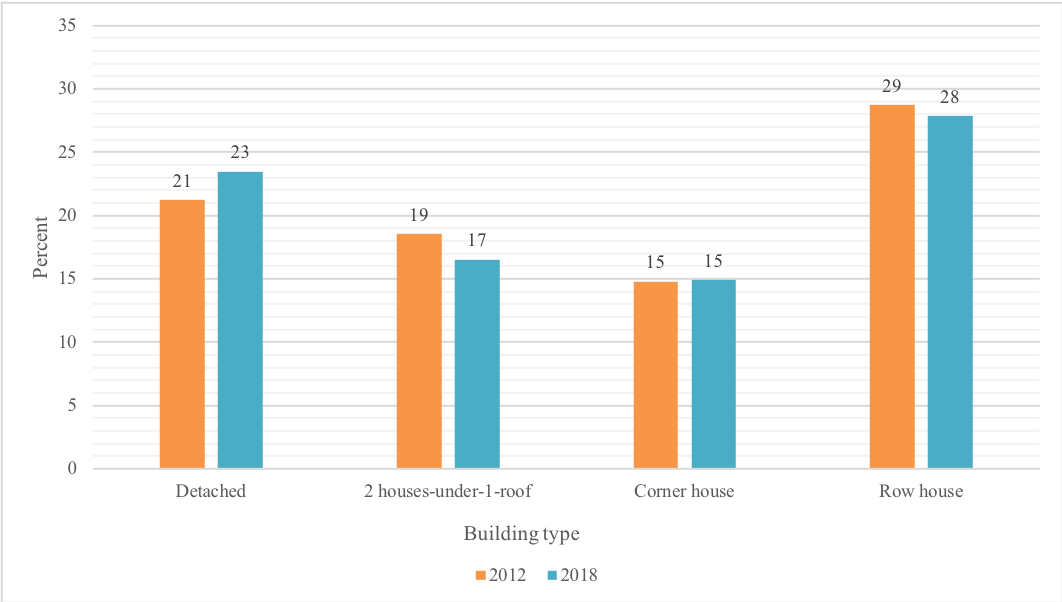
\includegraphics[width=14cm, height=7cm, clip, trim=4 4 4 4, clip]{buildingtype.PNG}
    \caption{Building types of "Woon energy module datasets of 2012 and 2018"}
    \label{fig:2}
\end{figure}

\begin{figure}[H]
    \centering
    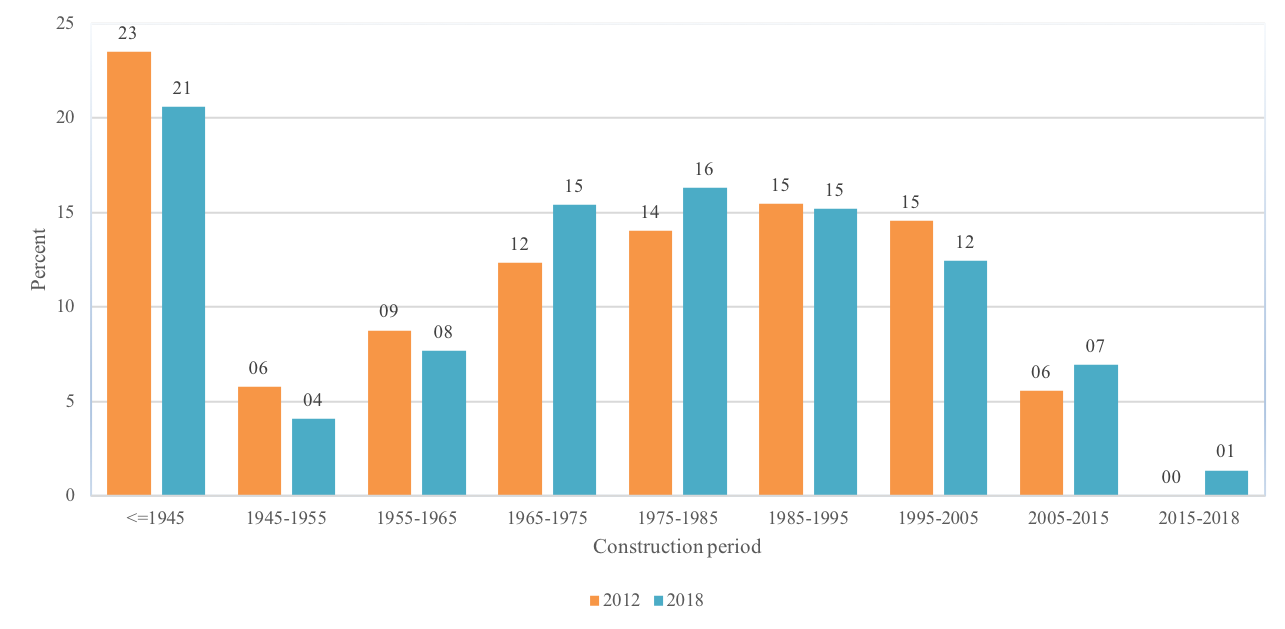
\includegraphics[width=14cm, height=7cm, clip, trim=4 4 4 4, clip]{constructionyear.PNG}
    \caption{Construction years of "Woon energy module datasets of 2012 and 2018"}
    \label{fig:3}
\end{figure}


With the assumption of consistency of the datasets at 2018 and 2012, the percentages of buildings with energy labels (G, F, E, and D) are decreased from 2012 to 2018, and instead the houses with energy labels (C, B, A, and A+), especially C and A, are increased. In both years, the majority of houses belongs to energy label "C" category. The number of houses of energy label "A" has the highest growth from 2012 to 2018, and the number of houses of energy label "F" has the highest drop from 2012 to 2018. All these changes show somehow the improvement in having more energy efficient houses in the Netherlands.

\begin{figure}[H]
    \centering
    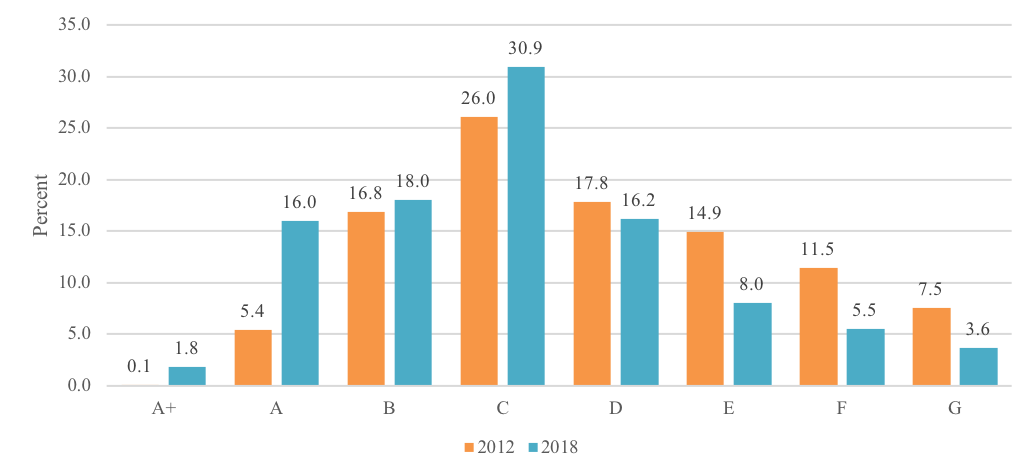
\includegraphics[width=15cm, height=6cm, clip, trim=4 4 4 4, clip]{Plabel.png}
    \caption{Distribution of buildings with different energy labels in "Woon energy module datasets of 2012 and 2018"}
    \label{fig:4}
\end{figure}


\subsubsection{Relationship between subsidies and costs on the energy efficiency measures}

Fig {\ref{fig:5}} shows a regression on the costs of energy efficiency measures and the impact of subsidies on the costs.Around point 3.5-4 (equal to 3,162.2-10,000 euros), the concentration of the subsidies are the highest. Also, the amount of subsidies are less than the costs for the majority of the cases. Only for two cases, the costs cover completely by subsidies. Also, in less than 10 cases, the subsidies are higher than the costs. As the costs increases, the subsidy rates are increased more rapidly. In 2012 and 2019, only 6\% and 13\% of householders received subsidies, respectively. The percentages of householders without subsidies did not change in both years. Approximately 50\% of householders did not recieve subsidies.       

\begin{figure}[H]
    \centering
    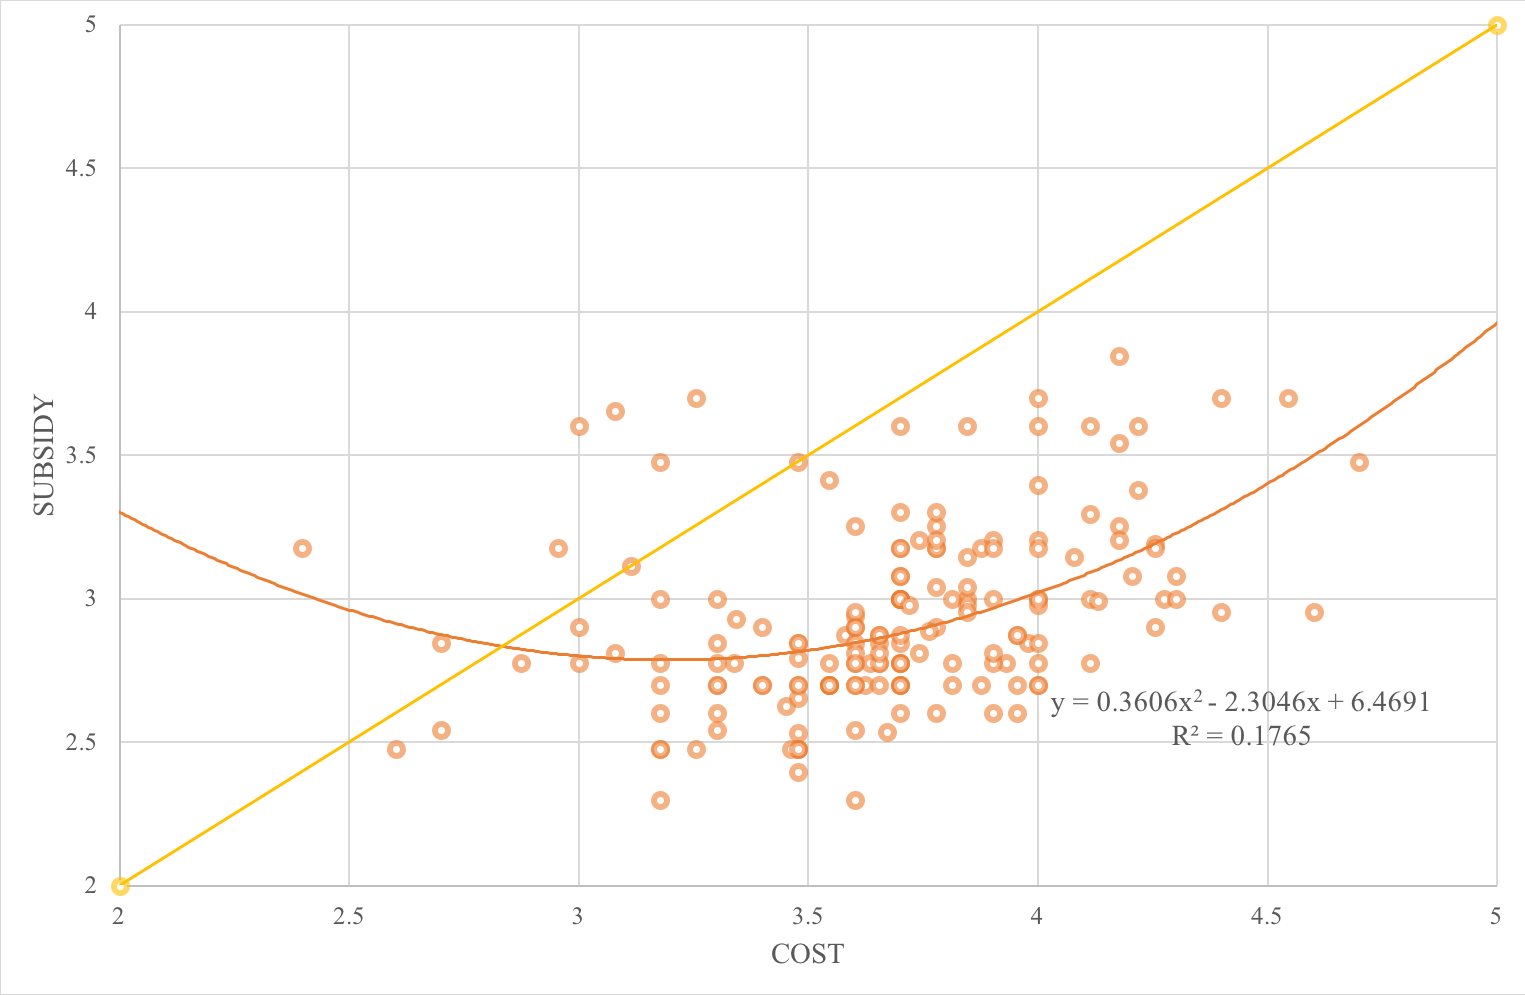
\includegraphics[width=15cm, height=10cm, clip, trim=4 4 4 4, clip]{SC.png}
    \caption{The costs and subsidies on the energy saving measures at 2018}
    \label{fig:5}
\end{figure}



\subsubsection{Renovators and potential renovators}

\noindent
\textbf{Renovators.} 55\% of householders have requested a specialised company or Do It Yourself companies to carry out the energy efficiency renovations. Considering the consistency of the two datasets (2012 and 2018), the number of renovators that have done the work by themselves is decreased from 22\% to 16\% (Fig \ref{fig:6}). 

\begin{figure}[H]
    \centering
    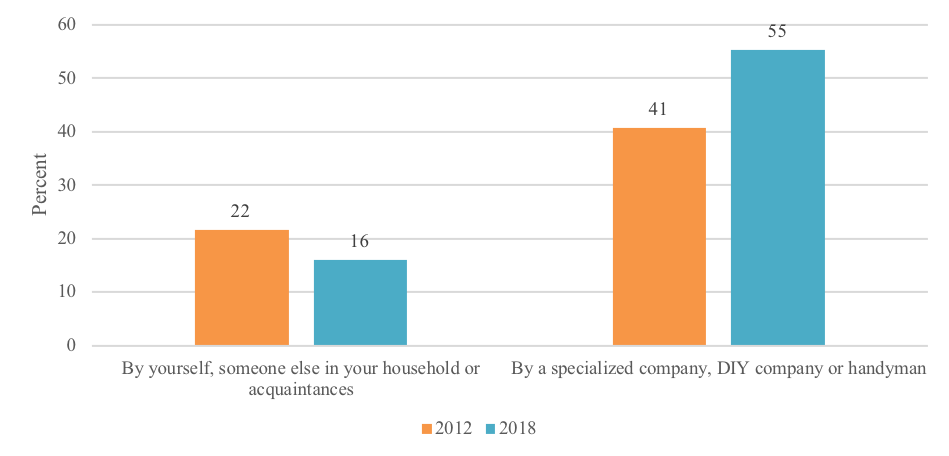
\includegraphics[width=12cm, height=6cm, clip, trim=4 4 4 4, clip]{donethework.PNG}
    \caption{The operators of energy efficiency renovation}
    \label{fig:6}
\end{figure}

Fig \ref{fig:7} shows the percentages of each energy-saving measures by renovators. Among these measures, double glazing has the highest percentages equal to 20.2\%. The central heating system is the second energy-saving measure that householders installed or replaced. The lowest percentage belongs to the additional window for the building.

\begin{figure}[H]
    \centering
    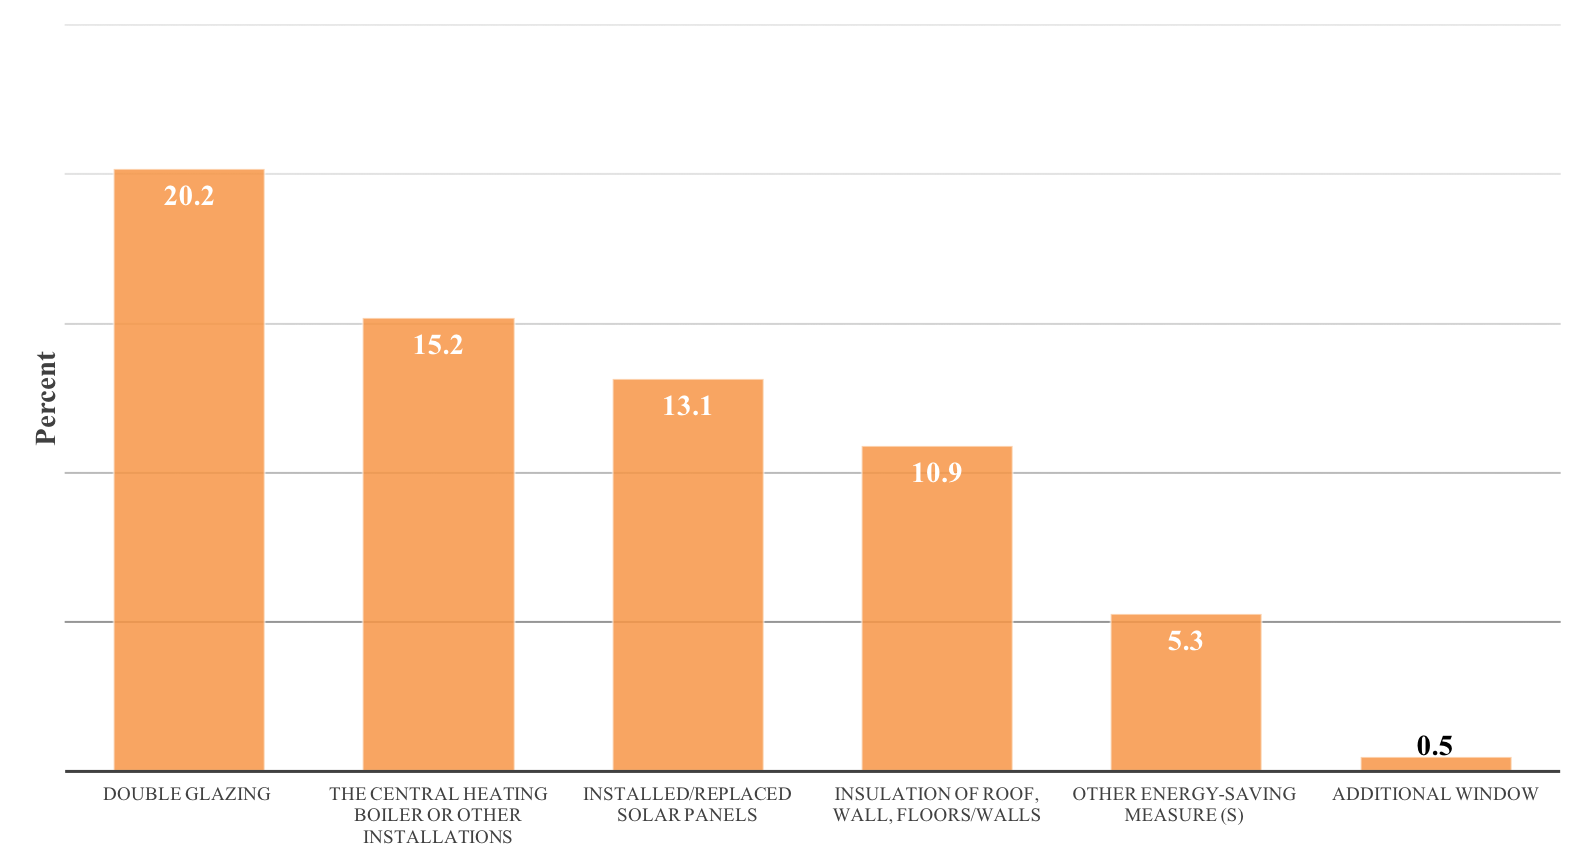
\includegraphics[width=12cm, height=6cm, clip, trim=4 4 4 25, clip]{ESMs.PNG}
    \caption{The percentages of renovators that have used different energy-saving measures}
    \label{fig:7}
\end{figure}

\subsubsection{Limitations of the database}


\subsection{Method of Analysis}

 The impact of behavioural factors are investigated for different energy efficiency measures. It helps to realise that besides to building characteristics which behaviour changes are important to implement different energy efficiency measures. Since, the dependent variable is binary (whether they have installed or will install the energy efficiency measures), the logistic regressions have been conducted. Five energy efficiency measures are the focus of our study. These energy saving measures are investigated for both renovators and potential renovators and in total, ten regressions have been conducted. The energy saving measures are double glazing, insulation (roof, wall, or floor), solar panel, and central heating boiler, and additional windows. The question was whether the householders implemented/planned to implement the specific energy saving measures in the last/next five years. The independent variables are the household and building characteristics, the behavioural factors, the drivers to implement energy saving measures, and the dependency with implementing different type of renovations.

Table \ref{tab:3} shows a logistic regression output in Statistical Package for the Social Sciences (SPSS). Coefficient B indicates the changes in log of the dependent variable for every one-unit change in an independent variable. Odds ratios (column exp(B)) explain the degree of association between dependent and independent variables and are used to compare the relative probabilities of the occurrence (chance criterion) of the renovation, given the presence of variable such as behavioural factors. For the variables with categories, generally the chance criterion is compared with the reference category. Binary variables can be seen as category variables with only two categories. The percentages of selecting the category $j$ by respondents can be calculated using the chance criterion $(exp(B_j)/(\sum^n_{i=1} exp(B_i))\times$100. A Wald test demonstrates the significance of each coefficient in the regression.

\begin{table}[H]
\caption{SPSS outputs for logistic regression}
\centering
\footnotesize
\begin{tabular}{@{}lllllll@{}}
\toprule
Independent variables & B & S.E. & Wald & df & Sig. & Exp(B) \\ \midrule
Constant &  &  &  &  &  &  \\ \bottomrule
\end{tabular}
\label{tab:3}
\end{table}

\noindent
There are some assumptions in conducting logistic regressions, including the binary dependent variable, not having multicollinearity between independent variables, and a large sample size. Validity of the multicollinearity 
assumption is  verified by calculating the Variance Inflation Factors (VIF). The VIF = 2.5 is the initial point of concern and VIF\textgreater10 shows multicollinearity \citep {midi2010}. The VIF for ten regressions are presented in Table \ref{tab:4}. There is no serious multicollinearity between the independent variables in the sample.

\begin{table}[H]
\caption{Multicollinearity tests in 10 regressions}
\footnotesize
\centering
\begin{tabular}{@{}lc@{}}
\toprule
Regression & max VIF \\ \midrule
\multicolumn{2}{c}{Renovators} \\ \midrule
Double glazing &  \\
Insulation &  \\
Solar panel &  \\
Central heating boiler & \\\midrule
\multicolumn{2}{c}{Potential renovators} \\ \midrule
Double glazing &  \\
Insulation &  \\
Solar panel &  \\
Central heating boiler & \\ \bottomrule
\end{tabular}
\label{tab:4}
\end{table}

\noindent
Binary logistic regression model used to describe the relation between the dependent variable and independent variables is presented in \cref{eq:1}:
\begin{equation}
\begin{aligned}
Log \left(\frac{P_{\text{renovation}}}{(1-P_{\text{renovation}})} \right)=& \beta_0+\beta_1 X_{\text{households and buildings' characteristics}}+ \beta_2X_{\text{motivations for renovations}}\\
&\beta_3X_{\text{sources of information}}+\beta_4X_{\text{TCs barriers}}+\beta_5X_{\text{State of maintenance for each type}}
\end{aligned}
\label{eq:1}
\end{equation}

\noindent
where P is the probability of the events, and X represents independent variables. After estimation, the Omnibus tests of model coefficients and the Hosmer and Lemeshow test are applied to validate the models, as shown in Table \ref{tab:9}. The Omnibus test checks whether the model estimates the outcome with the explanatory variables better than without \citep {brant1990}. The Omnibus tests are statistically significant, and the models are better with explanatory variables than without. The Hosmer and Lemeshow test illustrates the goodness of fit, which is a significant factor for a good model.


\begin{table}[H]
  \centering
  \footnotesize
  \caption{Assessing the regressions regarding the goodness of fit}
    \begin{tabular}{p{5em}|c|c|c|c|c|c|c}
    \toprule
      & \multicolumn{3}{c|}{Omnibus Tests of Model Coefficient} & \multicolumn{3}{c|}{Hosmer and Lemeshow Test} & R2\\
\cmidrule{2-7}    
\multicolumn{1}{r|}{} & \multicolumn{1}{c|}{Chi-square} & \multicolumn{1}{c|}{df} & \multicolumn{1}{c|}{Sig.} & \multicolumn{1}{c|}{Chi-square} & \multicolumn{1}{c|}{df} & \multicolumn{1}{c|}{Sig.} &  \\
    \midrule
    \multicolumn{8}{c}{Renovators} \\
    \midrule
    Double glazing & 132.871 & 33    & 0.000 & 13.021 & 8     & 0.111 & 0.223 \\
    
    Insulation & 143.216 & 27     & 0.000 & 8.465 & 8     & 0.389 & 0.231 \\
    
    Solar panel & 127.343 & 31     & 0.000 & 2.664 & 8     & 0.954 & 0.192 \\
    Central heating boiler & 127.343 & 31     & 0.000 & 2.664 & 8     & 0.954 & 0.192\\  \midrule
    \multicolumn{8}{c}{Potential renovators} \\
    \midrule
    Double glazing & 41.174 & 23     & 0.011 & 9.366 & 8     & 0.312 & 0.143 \\

    Insulation & 99.938 & 35    & 0.000 & 11.532 & 8     & 0.173 & 0.357 \\
    
    Solar panel & 109.455 & 33     & 0.000 & 8.887 & 8     & 0.352 & 0.336 \\
    Central heating boiler & 109.455 & 33     & 0.000 & 8.887 & 8     & 0.352 & 0.336 \\
 
    \bottomrule
    \end{tabular}
  \label{tab:5}
\end{table}

\section{Results}

\subsection{Expected vs. actual values by homeowners}

\subsubsection{Energy Label}

In the Woon energy module 2019, householders mention the expectation on the energy labels of their houses. The actual energy labels are extracted from other sources. Fig \ref{fig:8} shows the number of people that has the actual and expected energy labels in different categories. For instance, the number of people that has actual energy label of "C" and expected energy label of "G" is equal to 14. The number of people that expect correctly the energy label "C" is equal to 241. The labels that have the highest percentages on the correct expected energy labels are "C" and "A". The second ranking belongs to energy label "B". The energy label "E", "F", and "G" are the ones with the low expectations on the correct energy labels, and "F" has the lowest one. For these energy labels (E, F, and G), the householders expect higher energy labels than what they actually have. A considerable amount of householders confuse between energy labels "D" and "C". In total, the number of householders that expected higher energy labels, e.g. expected = "A" and actual = "B", are higher than the ones who expected lower energy labels compared to the actual ones. There are less than 3 householders that expect five energy label differences with the actual ones. 

\begin{figure}[H]
    \centering
    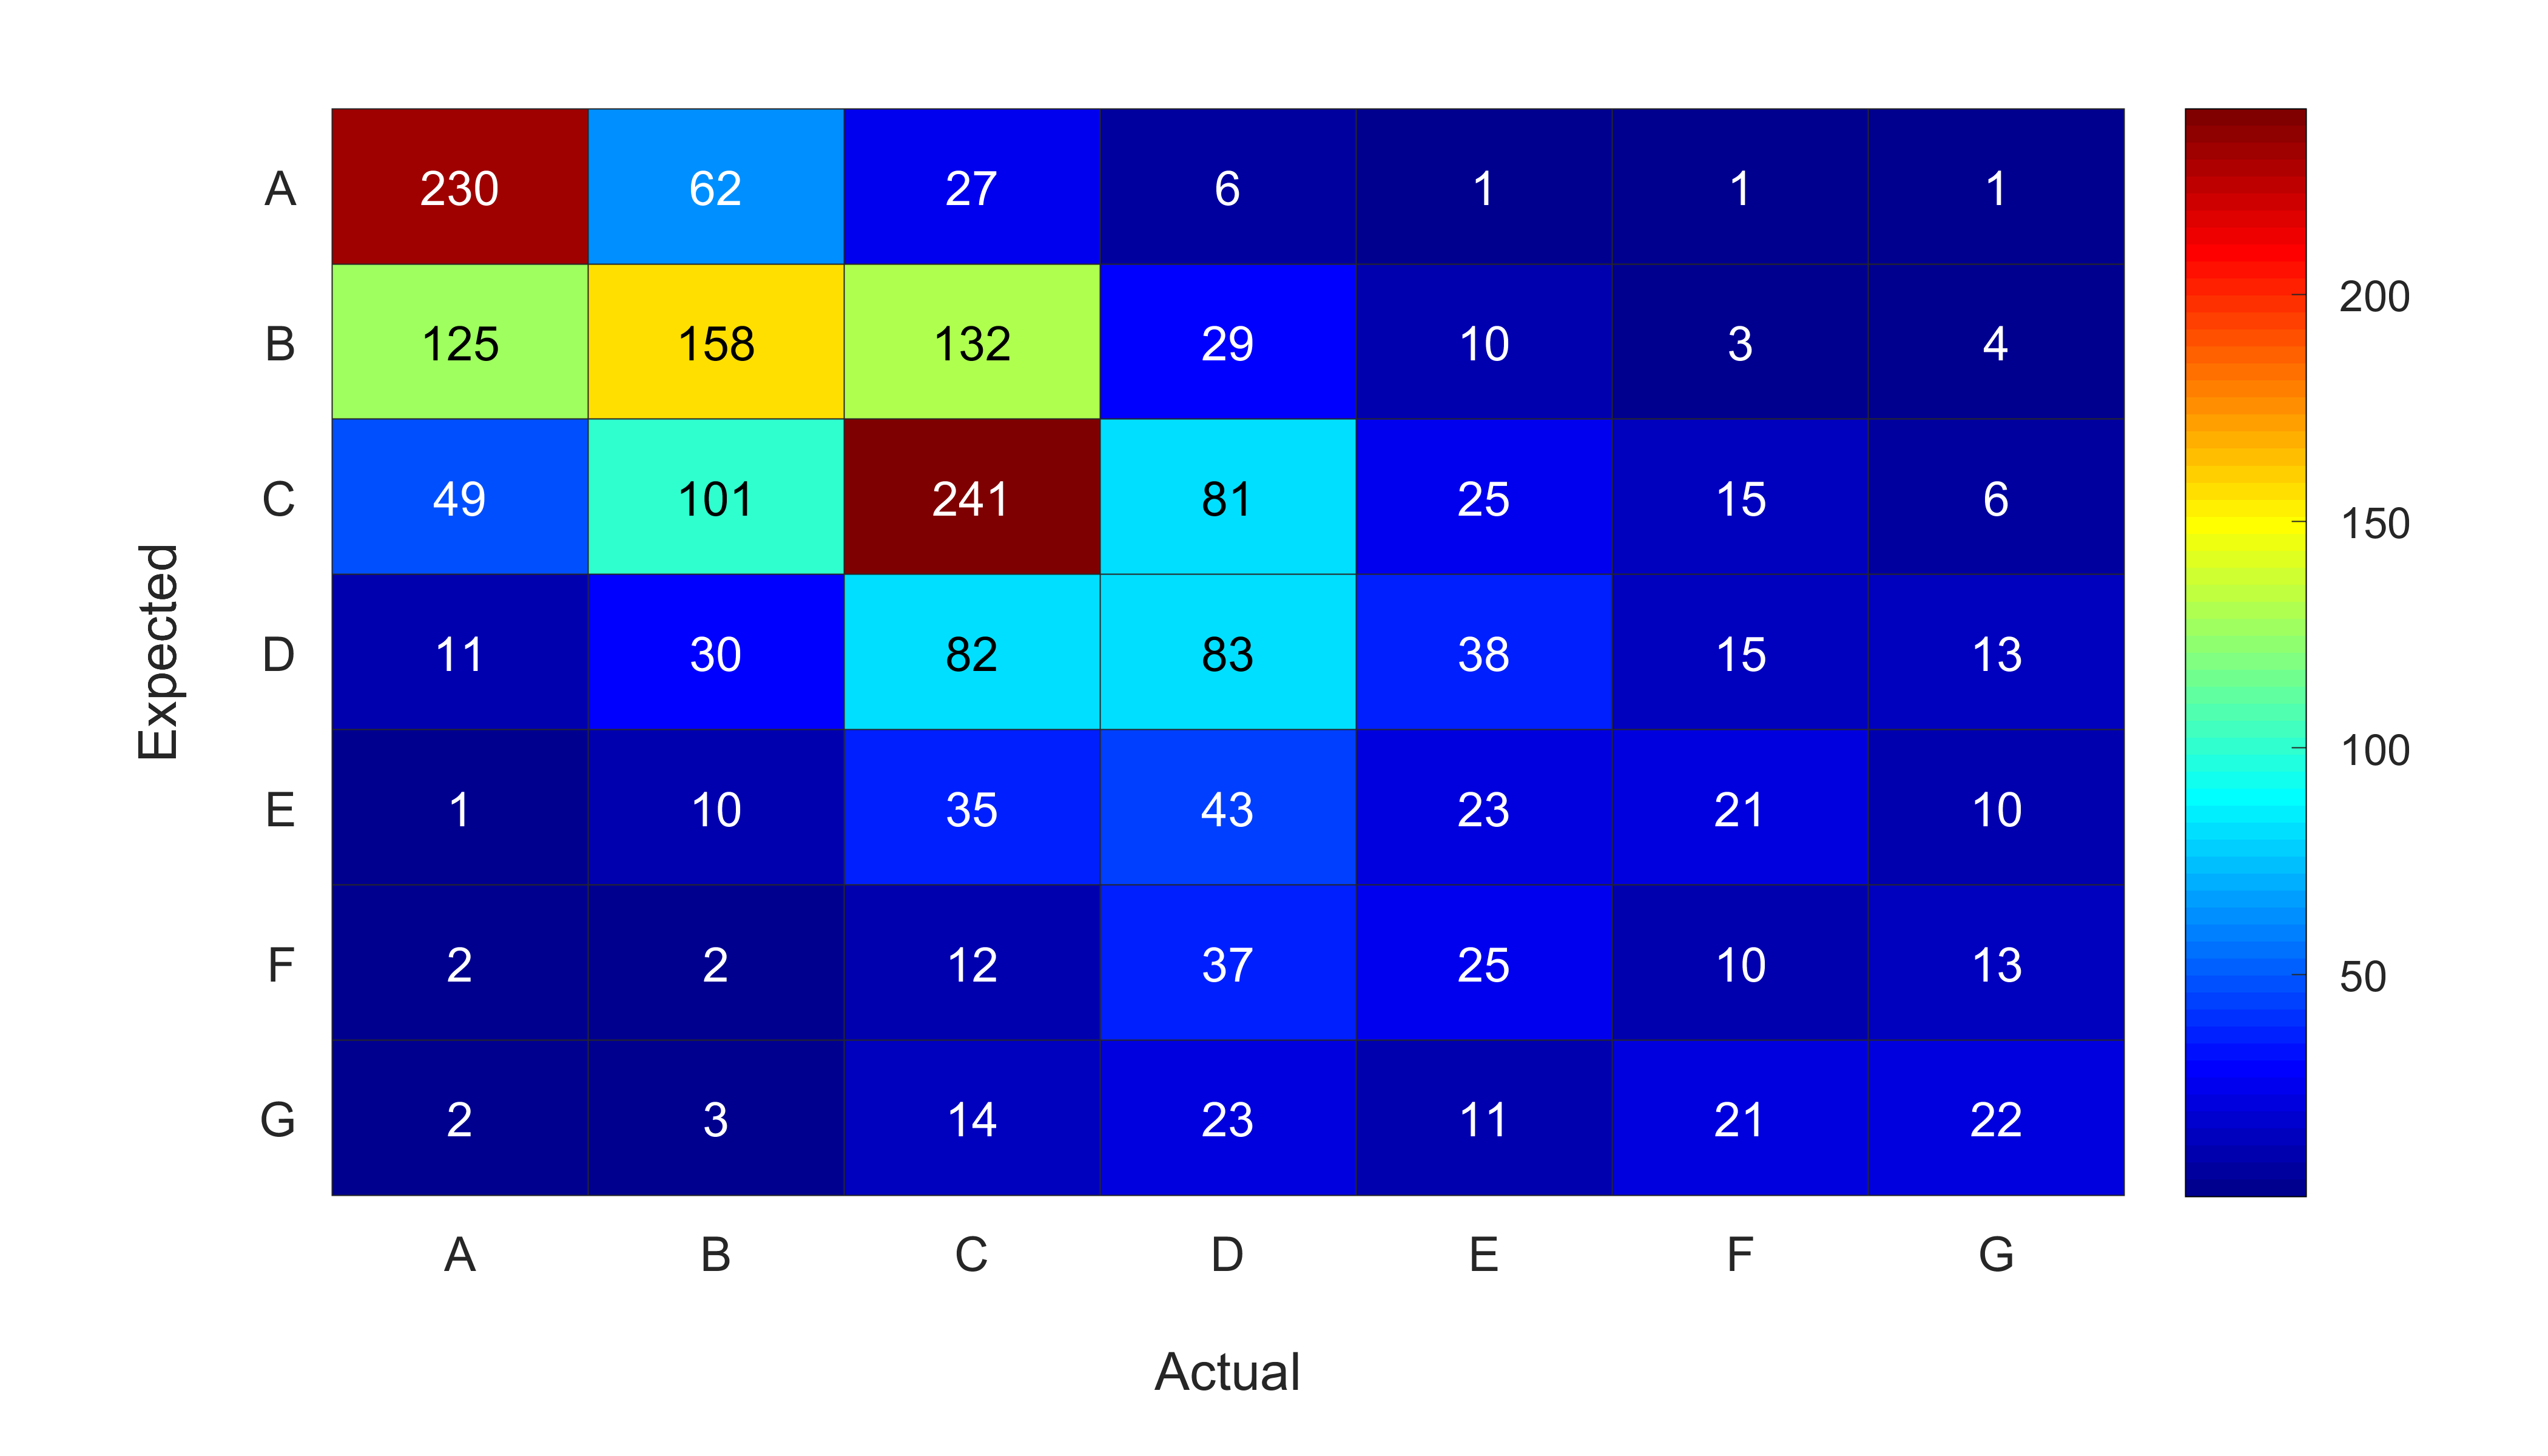
\includegraphics[width=15cm, height=10cm]{EnergyLabel.png}
    \caption{Heatmap chart of actual and expected energy labels}
    \label{fig:8}
\end{figure}

\subsubsection{Electricity consumption}

Fig \ref{fig:9} shows additional indicator regarding the householders expectation and actual values of electricity consumption. The highest number of householders belongs to the group that use electricity within the average of electricity consumption and expect that they use on average. The second ranking are for householders that use the energy higher than the average, however they expect that their electricity consumption is lower than average. A considerable amount of householders in the higher category are expected that their electricity consumption is on average. Also, a huge number of householders that use the electricity equal to average group, their expectation is on lower category of electricity consumption. The householders that belong to "much higher" and "much lower" actual electricity consumption seems to have the highest unrealistic expectations of their electricity consumption. In total, householders expect less electricity consumption compared to the actual ones. 

\begin{figure}[H]
    \centering
    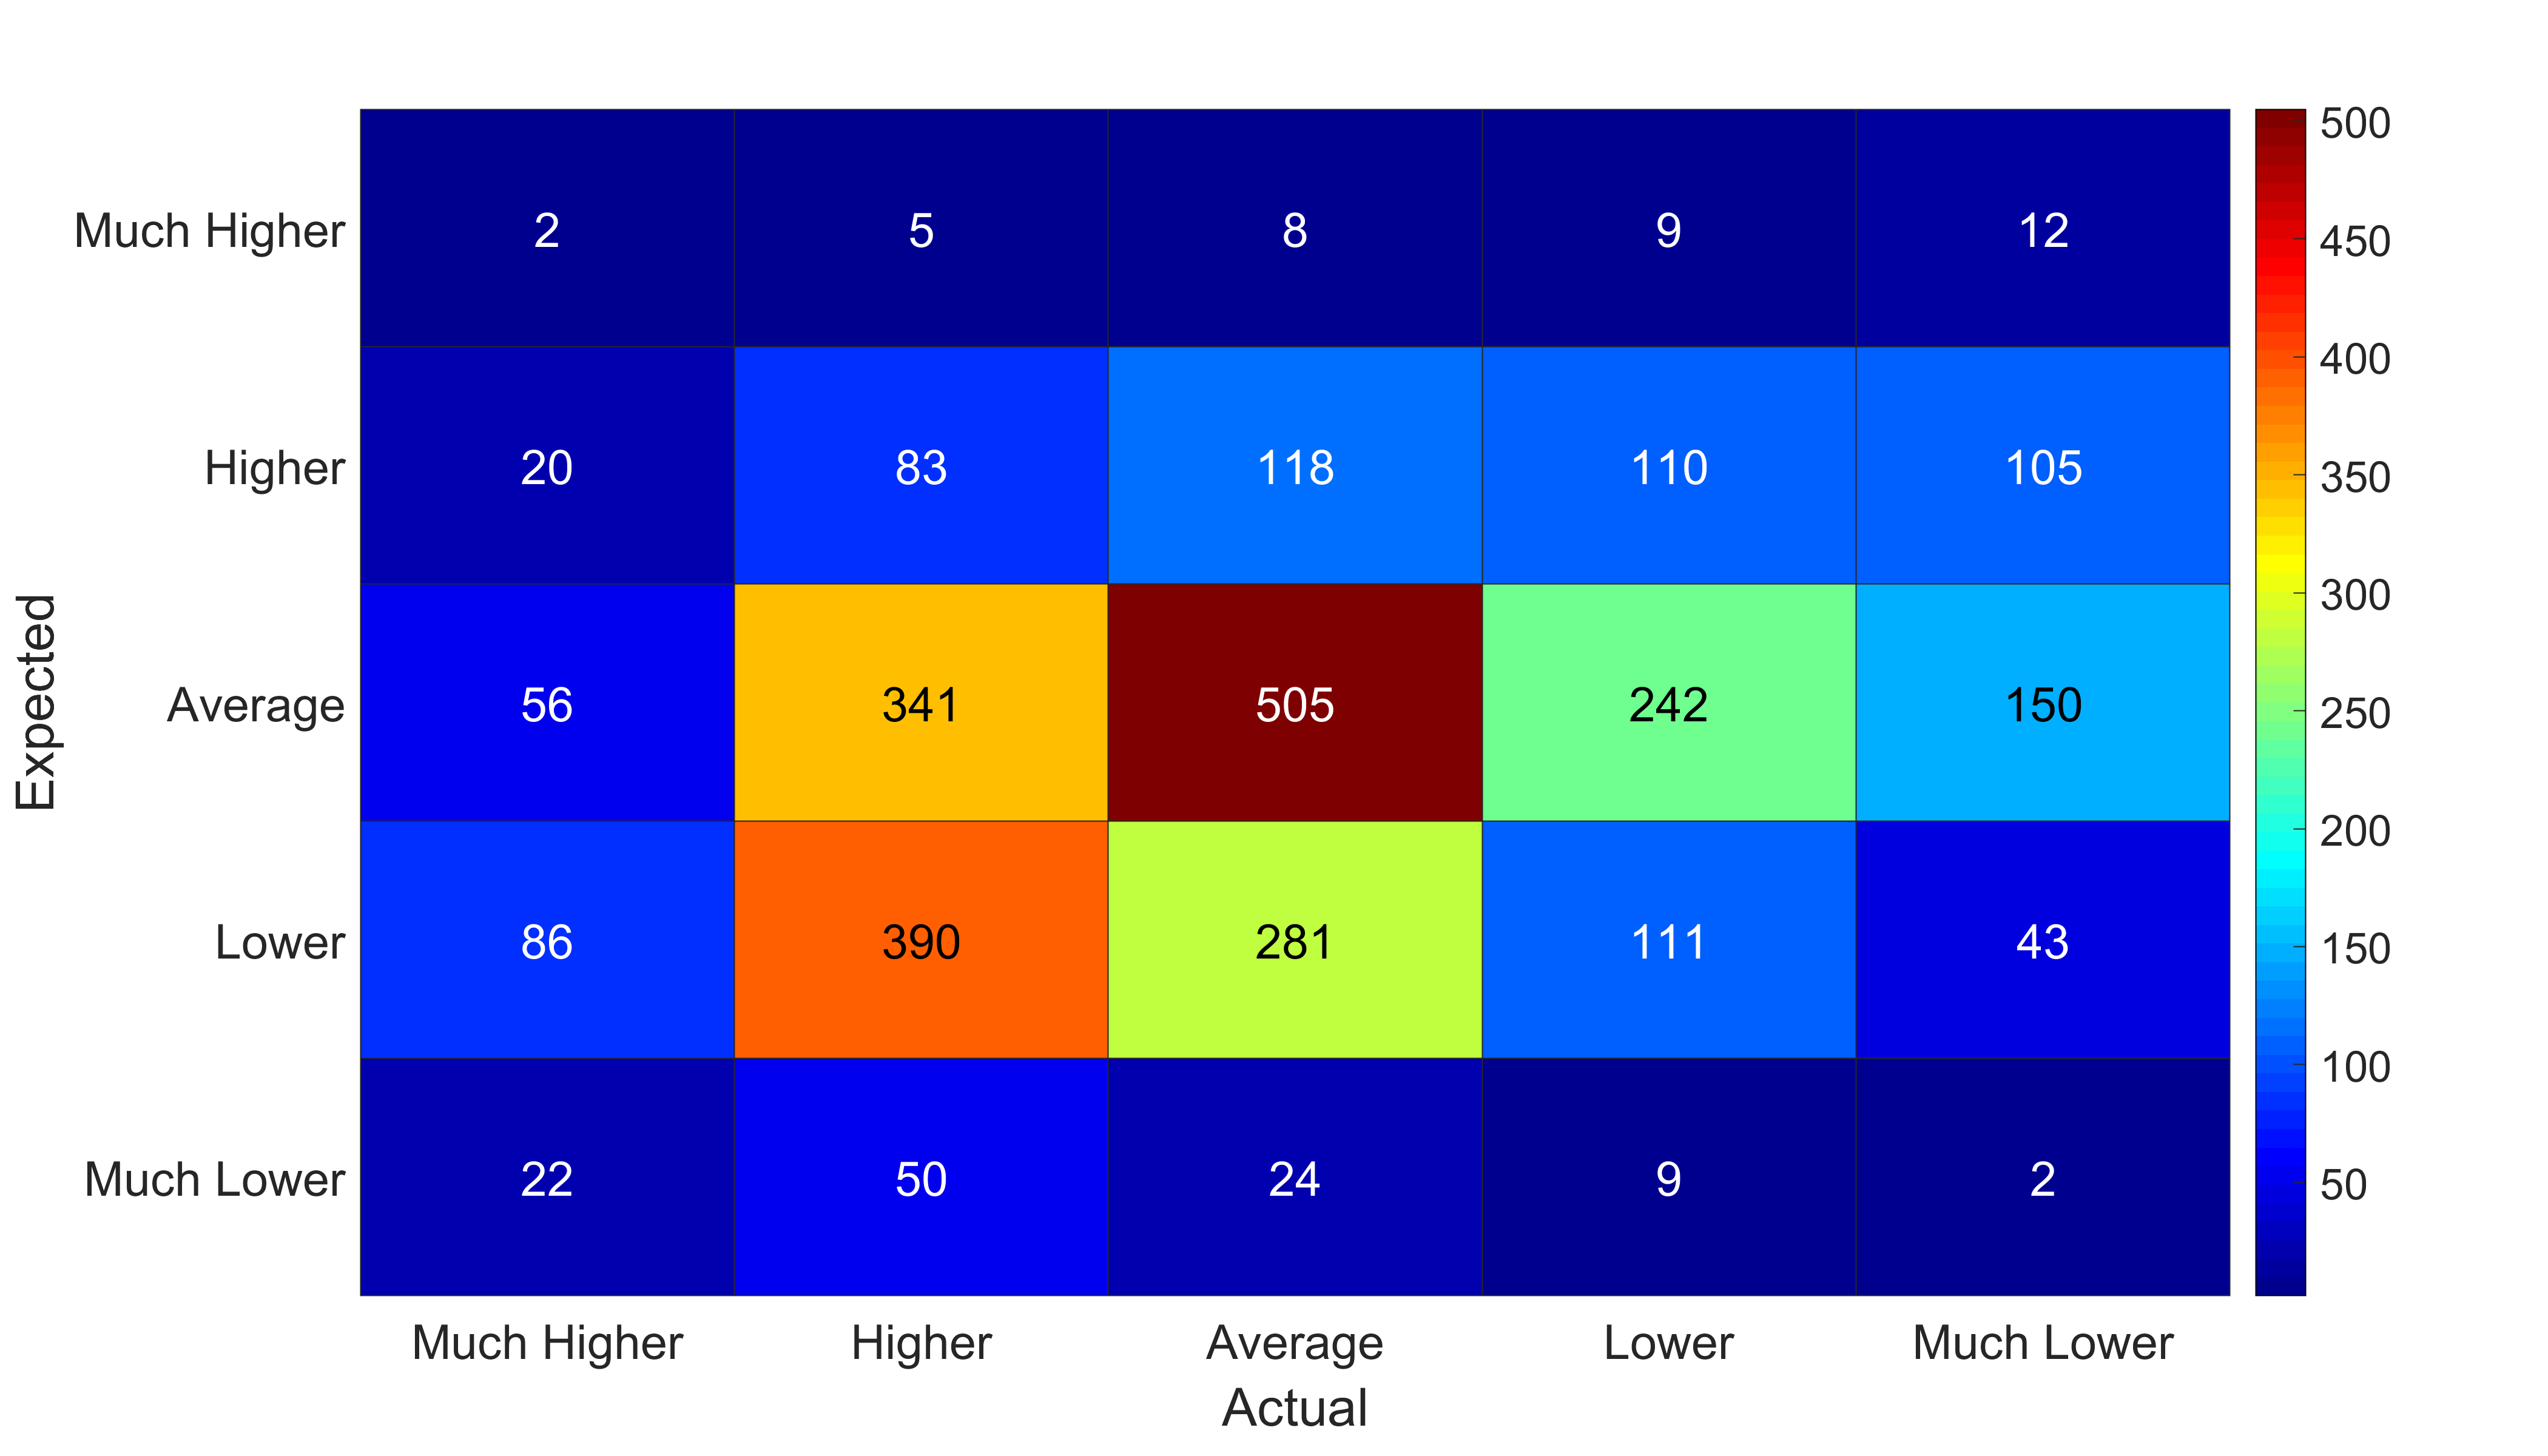
\includegraphics[width=15cm, height=9cm]{Electricity.png}
    \caption{Heatmap chart of actual and expected electricity consumption}
    \label{fig:9}
\end{figure}


\subsubsection{Gas consumption}

Fig \ref{fig:10} shows the results for the gas consumption similar to electricity. The highest number of correct expectations belong to the householders with average gas consumption. The second ranking is for people that consume higher than average in reality. However, their expectation is surprisingly "lower than average". The next highest number is again for the same group, i.e. that in reality consume higher than average, however, their expectation of gas consumption is on average. After these higher gas consumers, the householder group has the highest number in which in reality consume on average, their expectation is that they consume less than average.  The considerable number of householders think that they consume gas on average, however, in reality, they consume lower than average. In total, householders expect less gas consumption compared to the actual ones. 


\begin{figure}[H]
    \centering
    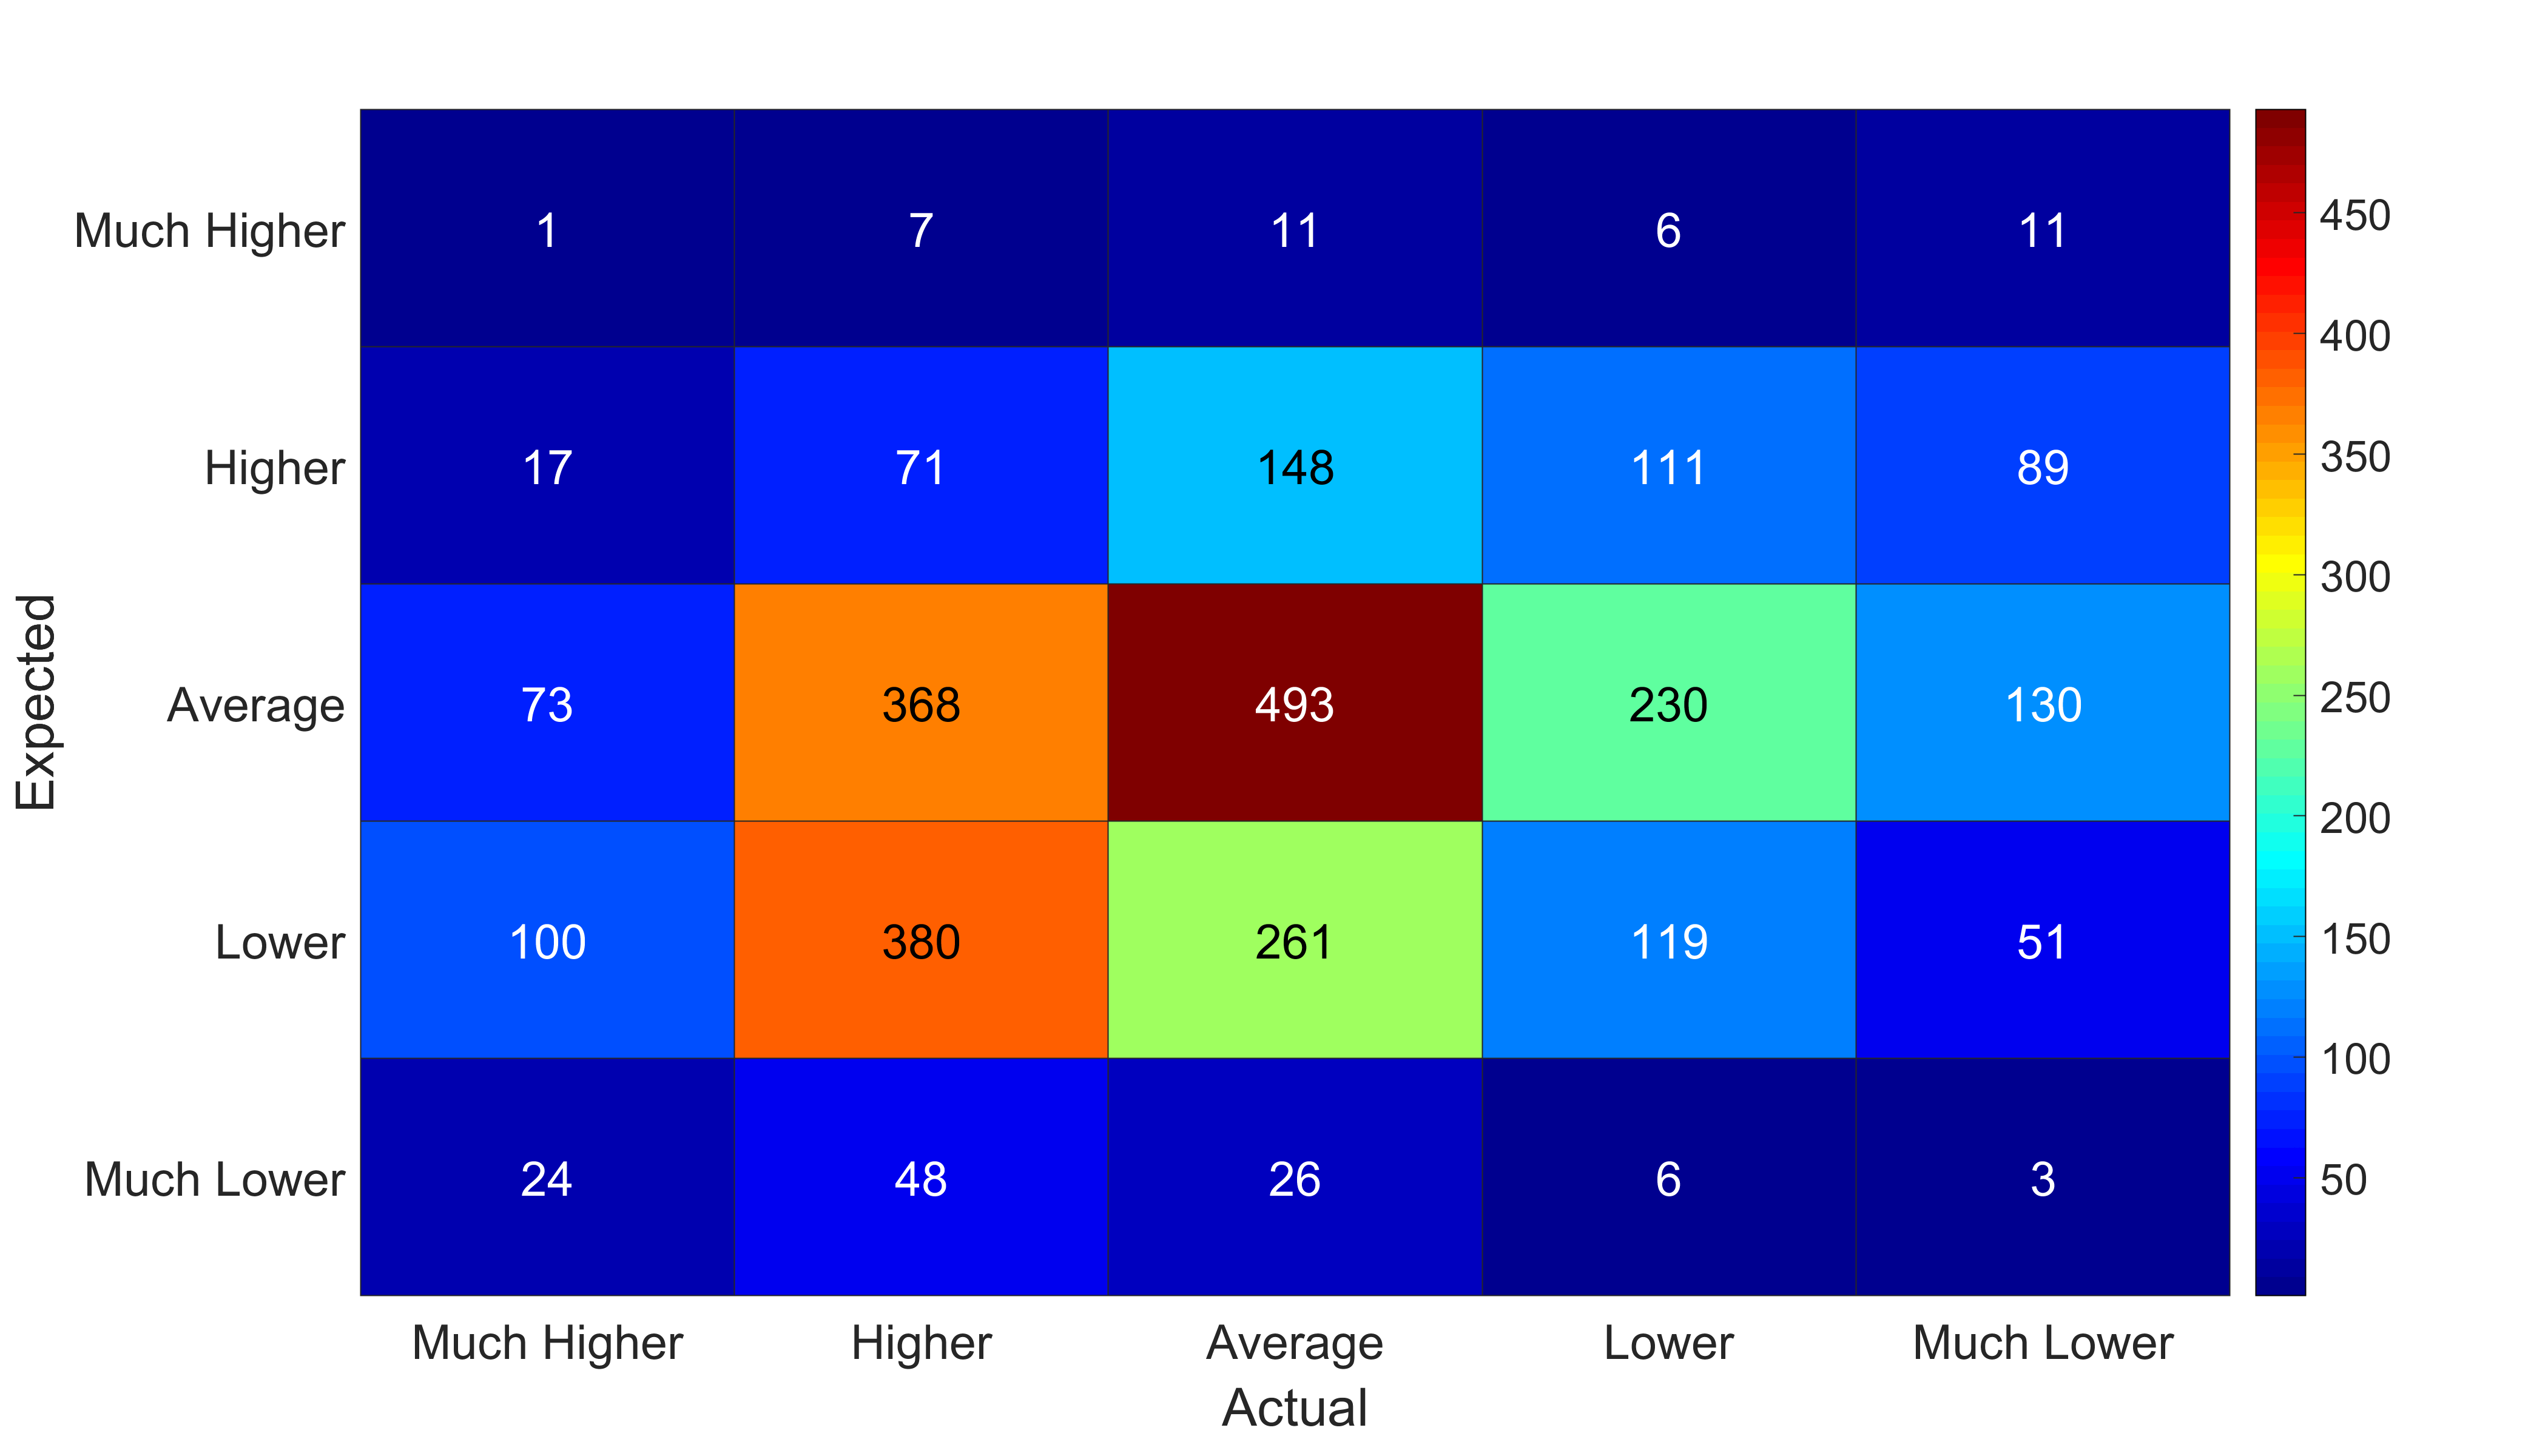
\includegraphics[width=15cm, height=9cm, clip]{Gas.png}
    \caption{Heatmap chart of actual and expected gas consumption}
    \label{fig:10}
\end{figure}


\subsection{Renovators}

\subsubsection{Energy saving measure: Double glazing}

Double glazing started to be used extensively in the 1980s and originally is invented to keep the building warm in the UK \citep{george1884}. Table (\ref{tab:6}) shows the logistic regression for influencing factors on the implementation of double glazing by householders. The construction years of (1985-1995) and (1995-2005) have the significant coefficients. The buildings before 1945 have higher probability to install double glazing compared to these two periods. This is expected since the double glazing did not exist widely in the old days. The 2 under 1 roofs buildings have installed more double glazing compared to detached house, and the reason is unclear. The householders with three and four members have higher probability to install the double glazing compared to single householders. The chance is 1.6 and 2.3, respectively. 

As mentioned by \citep{ebrahimi2019}, behavioural factors include the drivers since it shows the main reasons of making a more energy efficient houses. The coefficient of the drivers indicates that householders mainly install the double glazing to maintain the house, to reduce noise, and lower energy bills. These results are based on the larger values of Wald test compared to other significant drivers. 66\%, 37\%, and 36\% of householders mentioned them as the main reasons. Additionally, "to increase the value of the house" and "to have a more pleasant house" are the other important drivers. The relations of implementing double glazing with other types of non-energy-efficient-renovations are investigated to promote the energy efficient measures with the relevant renovations. The double glazing indicates significant relations to few types of renovations. The main identified/ the most significant one is  "repaired/replaced the window frames" and 80\% of respondents mentioned that they conducted double glazing with this type of renovation. The other significant ones are "windows installation" and "An extension made". Approximately 75\% of householders conduct these types of renovations together with double glazing.    

\begin{footnotesize}
\begin{longtable}[c]{@{}lllllll@{}}
\caption{Logistic regression for influencing factors on double glazing}
\label{tab:6}\\
\toprule
Variables                                                                                                & B      & S.E. & Wald   & df & Sig. & Exp(B) \\* \midrule
\endfirsthead
%
\multicolumn{7}{c}%
{{\bfseries Table \thetable\ continued from previous page}} \\
\toprule
Variables                                                                                                & B      & S.E. & Wald   & df & Sig. & Exp(B) \\* \midrule
\endhead
%
\bottomrule
\endfoot
%
\endlastfoot
%
\begin{tabular}[c]{@{}l@{}}construction years: \\ \textless{}1945\end{tabular}                           &        &      & 43.467 & 7  & .000 &        \\
1945-1955                                                                                                & -.404  & .383 & 1.116  & 1  & .291 & .667   \\
1955-1965                                                                                                & -.124  & .267 & .216   & 1  & .642 & .883   \\
1965-1975                                                                                                & .047   & .214 & .048   & 1  & .826 & 1.048  \\
1975-1985                                                                                                & .133   & .212 & .394   & 1  & .530 & 1.142  \\
1985-1995                                                                                                & -.990  & .260 & 14.525 & 1  & .000 & .371   \\
1995-2005                                                                                                & -2.017 & .426 & 22.447 & 1  & .000 & .133   \\
2005-2018                                                                                                & .073   & .435 & .028   & 1  & .867 & 1.075  \\
\begin{tabular}[c]{@{}l@{}}Type of single-family houses\_\\ (1) detached houses\end{tabular}             &        &      & 8.434  & 3  & .038 &        \\
(2) 2 under 1 roof                                                                                       & .408   & .205 & 3.964  & 1  & .046 & 1.504  \\
(3) Row corner houses                                                                                    & -.119  & .213 & .313   & 1  & .576 & .888   \\
(4) Row middle houses                                                                                    & -.141  & .189 & .558   & 1  & .455 & .868   \\
Number of people-1                                                                                       &        &      & 12.095 & 4  & .017 &        \\
2                                                                                                        & .280   & .227 & 1.523  & 1  & .217 & 1.324  \\
3                                                                                                        & .474   & .284 & 2.787  & 1  & .095 & 1.607  \\
4                                                                                                        & .842   & .263 & 10.272 & 1  & .001 & 2.320  \\
\textgreater{}5                                                                                          & .453   & .342 & 1.750  & 1  & .186 & 1.573  \\
\begin{tabular}[c]{@{}l@{}}Driver (s)-\\ (1) To maintain.\end{tabular} & -.516  & .155 & 11.098 & 1  & .001 & .597   \\
(2) To reduce noise.                                                                                         & -.554  & .227 & 5.959  & 1  & .015 & .574   \\
\begin{tabular}[c]{@{}l@{}}(3) To have a pleasant house.\end{tabular}                                & -1.124 & .161 & 48.840 & 1  & .000 & .325   \\
\begin{tabular}[c]{@{}l@{}} (4) A lower energy bill.\end{tabular} & .670   & .158 & 17.895 & 1  & .000 & 1.955  \\
\begin{tabular}[c]{@{}l@{}}(5) To increase the value.\end{tabular}                             & -.708  & .176 & 16.149 & 1  & .000 & .493   \\

\begin{tabular}[c]{@{}l@{}}Relation with maintenance:\\ (1) Replaced/repaired the roof.\end{tabular}          & 1.362  & .246 & 30.694 & 1  & .000 & 3.903  \\
(2) Window installations.                                                                                & 1.144  & .363 & 9.948  & 1  & .002 & 3.139  \\
\begin{tabular}[c]{@{}l@{}}(3) An extension made.\end{tabular}                             & 1.163  & .393 & 8.753  & 1  & .003 & 3.200  \\
\begin{tabular}[c]{@{}l@{}}(4) Repaired/ replaced window frames.\end{tabular}                             & 1.452  & .238 & 37.111 & 1  & .000 & 4.272  \\
\begin{tabular}[c]{@{}l@{}}(5) Painted exterior/window frames.\end{tabular}  & .515   & .221 & 5.415  & 1  & .020 & 1.673  \\
Constant                                                                                                 & 1.911  & .652 & 8.606  & 1  & .003 & 6.763  \\* \bottomrule
\end{longtable}
\end{footnotesize}






\subsubsection{Energy saving measure: floor, roof and wall insulation}

Insulation does not only cut down the use of heating, ventilation, and air conditioning systems but also it helps to reduce the energy costs \citep{al2005}. Practitioners also emphasise insulation as the best way to prevent heat loss \citep{polreff19}. Table \ref{tab:7} shows the influencing factors on insulation of floor, roof, and wall of a building. The construction year is a significant factor, and the houses which built between (1955-1965), (1985-1995), and (1995-2005) are identified significant. The houses with the construction years of (1955-1965) are insulated 1.6 times more in compared to the ones before 1945. The reference buildings are insulated 2.5 and 3.6 times more compared to the ones at (1985-1995) and (1995-2005).

Among the behavioural factors, the main identified one is "Changing the behaviour deliberately to use less electricity". It means householders that change their behaviour toward electricity consumption has done more insulation for the houses. 40\% of the householders that changed their behaviour have done insulation.  Another significant behavioural factor is the awareness regarding the energy consumption. The specified question is "Whether the householders know how much they use gas/electricity per year." In this case, all the groups have significant coefficients and the comparison is difficult. However, the "Well aware" householders have the highest Wald test and it can be concluded that this group of householders insulated their houses more than the other two groups. The last category of behavioural factors are the drivers. Two main identified drivers are "to maintain" and "to improve ventilation/moisture problem". The percentages of householders that specified these drivers and insulated their houses are equal to 67.5\% and 41\%, respectively. The renovation package does not seem reasonable to be done with boiler installation. Therefore, the intrepation is not done. 

\begin{footnotesize}

\begin{longtable}[c]{@{}lllllll@{}}
\caption{Logistic regression for influencing factors on floor, roof and wall insulation}
\label{tab:7}\\
\toprule
Variables                                                                                        & B       & S.E.     & Wald   & df & Sig.  & Exp(B) \\* \midrule
\endfirsthead
%
\multicolumn{7}{c}%
{{\bfseries Table \thetable\ continued from previous page}} \\
\toprule
Variables                                                                                        & B       & S.E.     & Wald   & df & Sig.  & Exp(B) \\* \midrule
\endhead
%
\bottomrule
\endfoot
%
\endlastfoot
%
\begin{tabular}[c]{@{}l@{}}construction years:\\ \textless{}1945\end{tabular}                    &         &          & 27,860 & 7  & 0,000 &        \\
1945-1955                                                                                        & 0,017   & 0,363    & 0,002  & 1  & 0,963 & 1,017  \\
1955-1965                                                                                        & 0,451   & 0,247    & 3,326  & 1  & 0,068 & 1,570  \\
1965-1975                                                                                        & -0,063  & 0,217    & 0,083  & 1  & 0,773 & 0,939  \\
1975-1985                                                                                        & -0,139  & 0,227    & 0,374  & 1  & 0,541 & 0,870  \\
1985-1995                                                                                        & -0,917  & 0,293    & 9,810  & 1  & 0,002 & 0,400  \\
1995-2005                                                                                        & -1,292  & 0,401    & 10,378 & 1  & 0,001 & 0,275  \\
2005-2018                                                                                        & -19,769 & 4935,330 & 0,000  & 1  & 0,997 & 0,000  \\
\begin{tabular}[c]{@{}l@{}}Change in behaviour \\ toward electricity \\ consumption\end{tabular} & -0,430  & 0,207    & 4,298  & 1  & 0,038 & 0,650  \\
\begin{tabular}[c]{@{}l@{}}Awareness of energy \\ consumption:(1) Well\\ aware\end{tabular}      &         &          & 7,028  & 2  & 0,030 &        \\
(2) Aware                                                                                        & 0,355   & 0,175    & 4,126  & 1  & 0,042 & 1,426  \\
(3) Not aware                                                                                    & 0,471   & 0,197    & 5,734  & 1  & 0,017 & 1,602  \\
\begin{tabular}[c]{@{}l@{}}Driver (s)-\\ (1) To maintain.\end{tabular}        & 0,729   & 0,153    & 22,610 & 1  & 0,000 & 2,073  \\
\begin{tabular}[c]{@{}l@{}}(2) To improve ventilation/\\ moisture problems.\end{tabular}       & -0,374  & 0,186    & 4,028  & 1  & 0,045 & 0,688  \\
\begin{tabular}[c]{@{}l@{}}(3) To have a pleasant house.\end{tabular}                    & -1,252  & 0,185    & 45,831 & 1  & 0,000 & 0,286  \\
\begin{tabular}[c]{@{}l@{}}(5) Repaired/replaced\\ window frames.\end{tabular}                 & -0,532  & 0,204    & 6,761  & 1  & 0,009 & 0,588  \\
Constant                                                                                         & 0,376   & 0,490    & 0,590  & 1  & 0,443 & 1,456  \\* \bottomrule
\end{longtable}
\end{footnotesize}






\subsubsection{Energy saving measure: solar panels installed or replaced}

The US scientists invented the solar panel in 1992 \citep{wagner1992}. The original term is a photo-voltaic module which absorb the sunlight to produce electricity, and solar panel is more a daily term. Table (\ref{tab:8}) shows the influencing factors on installation of solar panels. The implementation of this energy efficient measure depend strongly on the energy labels of the houses. The exp(B) values indicates that as long as energy label decreases (From "A" to "B"), the probability of solar panel installation declines. As an example, the householders with energy label "A" have 2.6 times more probably to install the solar panels compared to energy label "B". 

The number of significant behavioural factors are more in compared to the double glazing and insulation. The first group of behavioural factors belongs to intentional behavioural changes by householders: (1) replacing the non-energy efficient devices with the efficient ones, (2) reducing the gas consumption. The householders that adopt these behavioural changes are 1.5 and 1.6 times more likely to install the solar panel for their houses. Second, the awareness of the householders regarding the energy consumption is also identified significantly. The well-aware households have the highest Wald test compared to the other groups and the coefficient is statistically significant. Third, perception of householders on electricity consumption compared to other householders is the other significant category of behavioural factors. The "very economical" householders on electricity consumption have 2.6 times higher chance to install the solar panel compared to the average group of householders on electricity consumption. The last category of behavioural factors are the drivers. The highest significant driver is "to have a more pleasant house" and "to maintain". 86\% and 72\% of respondents that installed the solar panels, mentioned these drivers as the main drivers to implement energy efficient measure. The other reasonable and significant drivers are "lowering the energy bills" and "protect the environment" with 10\% and 27\%. 

As expected, 76\% of householders asked an expert to install the solar panels instead of doing themselves. The installation of solar panels happened whenever the householders "Replaced/ repaired the roof" or "Replaced/repaired the windows frames. The 33\% and 29\% of householders that mentioned these two types of renovation, installed the solar panels. 68\% of householders did the boiler installation by experts rather than doing it themselves. 


\begin{footnotesize}
\begin{longtable}[c]{@{}lllllll@{}}
\caption{Logistic regression for influencing factors on solar panels (installed/replaced)}
\label{tab:8}\\
\toprule
Variables                                                                                                                                   & B      & S.E.  & Wald   & df & Sig.  & Exp(B) \\* \midrule
\endfirsthead
%
\multicolumn{7}{c}%
{{\bfseries Table \thetable\ continued from previous page}} \\
\toprule
Variables                                                                                                                                   & B      & S.E.  & Wald   & df & Sig.  & Exp(B) \\* \midrule
\endhead
%
\bottomrule
\endfoot
%
\endlastfoot
%
Energy labels \_ A and A+                                                                                                                   &        &       & 64,138 & 6  & 0,000 &        \\
B                                                                                                                                           & -0,963 & 0,257 & 14,011 & 1  & 0,000 & 0,382  \\
C                                                                                                                                           & -1,503 & 0,244 & 37,954 & 1  & 0,000 & 0,222  \\
D                                                                                                                                           & -1,932 & 0,331 & 34,138 & 1  & 0,000 & 0,145  \\
E                                                                                                                                           & -2,304 & 0,476 & 23,446 & 1  & 0,000 & 0,100  \\
F                                                                                                                                           & -1,945 & 0,550 & 12,523 & 1  & 0,000 & 0,143  \\
G                                                                                                                                           & -1,401 & 0,660 & 4,510  & 1  & 0,034 & 0,246  \\
\begin{tabular}[c]{@{}l@{}}Changing behaviour by replacing\\ devices that used a lot of energy\\ with energy-efficient devices.\end{tabular} & 0,414  & 0,198 & 4,382  & 1  & 0,036 & 1,513  \\
\begin{tabular}[c]{@{}l@{}}Changing behaviour by\\ deliberately used less gas\end{tabular}                                                  & 0,442  & 0,193 & 5,254  & 1  & 0,022 & 1,556  \\
\begin{tabular}[c]{@{}l@{}}Awareness of energy\\ consumption:\\ (1) Well aware\end{tabular}                                                 &        &       & 5,214  & 2  & 0,074 &        \\
(2) Aware                                                                                                                                   & -0,246 & 0,209 & 1,392  & 1  & 0,238 & 0,782  \\
(3) Not aware                                                                                                                               & -0,627 & 0,284 & 4,862  & 1  & 0,027 & 0,534  \\
\begin{tabular}[c]{@{}l@{}}Perception on electricity\\ consumption compared\\ to other households:\\ very economical\end{tabular}           &        &       & 9,688  & 3  & 0,021 &        \\
Economical                                                                                                                                  & -0,481 & 0,370 & 1,689  & 1  & 0,194 & 0,618  \\
Average                                                                                                                                     & -0,966 & 0,378 & 6,545  & 1  & 0,011 & 0,381  \\
Inefficient                                                                                                                                 & -0,793 & 0,586 & 1,831  & 1  & 0,176 & 0,452  \\
\begin{tabular}[c]{@{}l@{}}Driver (s)- (1) To maintain.\end{tabular}                                                   & 0,957  & 0,190 & 25,351 & 1  & 0,000 & 2,605  \\
\begin{tabular}[c]{@{}l@{}}(2) To reduce noise.\end{tabular}                                                                   & 0,879  & 0,481 & 3,341  & 1  & 0,068 & 2,410  \\
\begin{tabular}[c]{@{}l@{}}(3) To improve ventilation/ \\moisture problems.\end{tabular}                                              & 0,862  & 0,391 & 4,873  & 1  & 0,027 & 2,368  \\
\begin{tabular}[c]{@{}l@{}}(4) To have a more pleasant house.\end{tabular}                                                              & 1,915  & 0,207 & 85,244 & 1  & 0,000 & 6,787  \\
\begin{tabular}[c]{@{}l@{}}(5) A lower energy bill.\end{tabular}                                & -2,019 & 0,280 & 51,858 & 1  & 0,000 & 0,133  \\
\begin{tabular}[c]{@{}l@{}}(6) For the environment.\end{tabular}                                                                   & -0,980 & 0,223 & 19,298 & 1  & 0,000 & 0,375  \\
\begin{tabular}[c]{@{}l@{}}Renovation by experts\\ compared to DIY\end{tabular}                                                             & 1,197  & 0,256 & 21,832 & 1  & 0,000 & 3,310  \\
\begin{tabular}[c]{@{}l@{}}Relation with \\ maintenance:\\ (1) Replaced/repaired the roof.\end{tabular}                                   & -0,713 & 0,298 & 5,730  & 1  & 0,017 & 0,490  \\
\begin{tabular}[c]{@{}l@{}}(2) Repaired/ replaced\\ window frames\end{tabular}                                                            & -0,908 & 0,286 & 10,104 & 1  & 0,001 & 0,403  \\
Constant                                                                                                                                    & -6,519 & 1,395 & 21,853 & 1  & 0,000 & 0,001  \\* \bottomrule
\end{longtable}
\end{footnotesize}


\subsubsection{Energy saving measure: the central heating boiler/ other installations}

According to the study in Uk, 55\% of the energy bills is accounted for the boiler. New boilers recover more heat because of having larger heat exchangers. Also, this study shows replacing a "G" rated boiler with "A" rated one leads to 375 euro saving \citep{boiler19, Energy2019}. Table (\ref{tab:9}) shows the influencing factors on installation of the central heating boilers. The construction years play an important role and houses that are constructed between (1985-1995) and (1995-2005). The latter has 10.4 and the other one 10.4 and 4 times more likely to replace the central heating boiler compared to other houses (?). The second significant building characteristic is the energy label. In contrast to the solar panel, the houses with lower energy labels have higher probability to install/replace the boilers. The highest significant energy label is for energy label "E" with the energy labels "F", "D", and "G" as the successors. The installation of new boilers depends on the number of people in the buildings. The type of houses is also a significant variable. Among different types of houses, the row middle houses have a significant and higher probability to install/ replace the boilers compared to detached houses. The chance is 1.8 times higher than detached houses. The householders with three persons have the significant impact on boiler installation. 41\% of householders with three persons installed/replaced the boiler. 

Among the behavioural factors, changing deliberately the behaviour to gas consumption is significant variable. 40\% of householders that did this change in their behaviour are installed/ replaced a central heating boiler. Second significant behavioural factor is the perception of householders regarding electricity consumption compared to other householders. The householders that perceive inefficiency in electricity consumption are 4.5 times more likely to replace their boiler compared to efficient users of electricity consumption. The main identified driver is "to have a more pleasant house" and "For environment". 79\% and 76\% of respondents.



\begin{footnotesize}
\begin{longtable}[c]{@{}lllllll@{}}
\caption{Logistic regression for influencing factors on the central heating boiler}
\label{tab:9}\\
\toprule
Variables                                                                                                                              & B      & S.E.  & Wald   & df & Sig.  & Exp(B) \\* \midrule
\endfirsthead
%
\multicolumn{7}{c}%
{{\bfseries Table \thetable\ continued from previous page}} \\
\toprule
Variables                                                                                                                              & B      & S.E.  & Wald   & df & Sig.  & Exp(B) \\* \midrule
\endhead
%
\bottomrule
\endfoot
%
\endlastfoot
%
\begin{tabular}[c]{@{}l@{}}construction years:\\ \textless{}1945\end{tabular}                                                          &        &       & 40,434 & 7  & 0,000 &        \\
1945-1955                                                                                                                              & 0,332  & 0,527 & 0,396  & 1  & 0,529 & 1,393  \\
1955-1965                                                                                                                              & -0,447 & 0,447 & 0,999  & 1  & 0,317 & 0,640  \\
1965-1975                                                                                                                              & 0,293  & 0,345 & 0,720  & 1  & 0,396 & 1,340  \\
1975-1985                                                                                                                              & 0,237  & 0,366 & 0,419  & 1  & 0,518 & 1,267  \\
1985-1995                                                                                                                              & 1,411  & 0,395 & 12,741 & 1  & 0,000 & 4,102  \\
1995-2005                                                                                                                              & 2,345  & 0,462 & 25,727 & 1  & 0,000 & 10,434 \\
2005-2018                                                                                                                              & 1,085  & 0,869 & 1,559  & 1  & 0,212 & 2,959  \\
Energy labels: A and A+                                                                                                                &        &       & 27,226 & 6  & 0,000 &        \\
B                                                                                                                                      & 1,440  & 0,353 & 16,658 & 1  & 0,000 & 4,222  \\
C                                                                                                                                      & 1,748  & 0,383 & 20,779 & 1  & 0,000 & 5,743  \\
D                                                                                                                                      & 2,169  & 0,463 & 21,988 & 1  & 0,000 & 8,751  \\
E                                                                                                                                      & 2,421  & 0,536 & 20,426 & 1  & 0,000 & 11,254 \\
F                                                                                                                                      & 2,147  & 0,639 & 11,293 & 1  & 0,001 & 8,561  \\
G                                                                                                                                      & 1,859  & 0,782 & 5,648  & 1  & 0,017 & 6,416  \\
\begin{tabular}[c]{@{}l@{}}Type of single-family houses\_\\ (1) detached houses\end{tabular}                                           &        &       & 6,547  & 3  & 0,088 &        \\
(2) 2 under 1 roof                                                                                                                     & 0,175  & 0,280 & 0,391  & 1  & 0,532 & 1,192  \\
(3) Row corner houses                                                                                                                  & 0,471  & 0,286 & 2,712  & 1  & 0,100 & 1,602  \\
(4) Row middle houses                                                                                                                  & 0,603  & 0,254 & 5,611  & 1  & 0,018 & 1,827  \\
Number of people -1                                                                                                                    &        &       & 10,252 & 4  & 0,036 &        \\
2                                                                                                                                      & 0,037  & 0,275 & 0,018  & 1  & 0,894 & 1,037  \\
3                                                                                                                                      & -0,352 & 0,351 & 1,006  & 1  & 0,316 & 0,703  \\
4                                                                                                                                      & -0,798 & 0,345 & 5,350  & 1  & 0,021 & 0,450  \\
\textgreater{}5                                                                                                                        & -0,556 & 0,466 & 1,426  & 1  & 0,232 & 0,573  \\
\begin{tabular}[c]{@{}l@{}}Change in behaviour\\ toward gas consumption\end{tabular}                                                   & -0,395 & 0,197 & 4,022  & 1  & 0,045 & 0,674  \\

\begin{tabular}[c]{@{}l@{}}Perception on electricity \\ consumption compared\\ to other households:\\ (1) very economical\end{tabular} &        &       & 16,093 & 3  & 0,001 &        \\
(2) Economical                                                                                                                         & 0,402  & 0,648 & 0,385  & 1  & 0,535 & 1,495  \\
(3) Average                                                                                                                            & 1,128  & 0,642 & 3,088  & 1  & 0,079 & 3,089  \\
(4) Inefficient                                                                                                                        & 1,498  & 0,735 & 4,151  & 1  & 0,042 & 4,473  \\
\begin{tabular}[c]{@{}l@{}}Driver (s)-\\(1) To maintain.\end{tabular}                                                 & -2,762 & 0,296 & 87,108 & 1  & 0,000 & 0,063  \\
\begin{tabular}[c]{@{}l@{}}(2) To improve ventilation/\\moisture problems.\end{tabular}                                             & 1,043  & 0,401 & 6,750  & 1  & 0,009 & 2,837  \\
\begin{tabular}[c]{@{}l@{}}(3) To have a more\\ pleasant house.\end{tabular}                                                          & 1,302  & 0,210 & 38,359 & 1  & 0,000 & 3,677  \\
\begin{tabular}[c]{@{}l@{}}(4) For environment.\end{tabular}                                                              & 1,157  & 0,209 & 30,759 & 1  & 0,000 & 3,182  \\
\begin{tabular}[c]{@{}l@{}}(5) Increase the house value. \end{tabular}                                                & 0,565  & 0,247 & 5,215  & 1  & 0,022 & 1,759  \\
\begin{tabular}[c]{@{}l@{}}Renovation by experts\\ compared to DIY\end{tabular}                                                        & 0,779  & 0,259 & 9,079  & 1  & 0,003 & 2,179  \\

\begin{tabular}[c]{@{}l@{}}Relation with maintenance:\\ (1) Replaced/repaired the roof\end{tabular}                                    & -1,424 & 0,328 & 18,861 & 1  & 0,000 & 0,241  \\
\begin{tabular}[c]{@{}l@{}}(2) Repaired/replaced window frames\end{tabular}                                                       & -1,311 & 0,308 & 18,141 & 1  & 0,000 & 0,270  \\
\begin{tabular}[c]{@{}l@{}}(3) Painted the exterior/\\ the window frames\end{tabular}                               & -0,458 & 0,222 & 4,237  & 1  & 0,040 & 0,633  \\
Constant                                                                                                                               & -8,462 & 1,354 & 39,084 & 1  & 0,000 & 0,000  \\* \bottomrule
\end{longtable}


\end{footnotesize}



\subsection{Potential renovators}


\subsubsection{Energy saving measure: Double glazing}

Table (\ref{tab:10}) shows the influencing factors on double glazing for potential renovators. The energy labels have the significant coefficients among the building characteristics. The most significant energy label is "G" that the householders with this energy label will plan 5.3 times more likely to install double glazing compared to energy labels (A and A+). After "G", the energy labels "F" and "D"  have the highest probability by householders to install double glazing in the future. 

Regarding the behavioural factors, 38\% of householders that mentioned they have deliberately change their behaviours by reducing the gas consumption are planning to do double glazing. Among the drivers, "to have a more pleasant house" and "to reduce noise" are the main identified ones. 76\% and 69\% of householders that mentioned the importance of these drivers are planning to install double glazing in the next two years. "To improve ventilation" and "to make the property more saleable" are the second important groups of drivers for potential renovators. Approximately, 63\% of householders that mentioned these drivers importantly, are planning to install double glazing. 


\begin{footnotesize}

\begin{longtable}[c]{@{}lllllll@{}}
\caption{Logistic regression for influencing factors on double glazing (potential renovators)}
\label{tab:10}\\
\toprule
Variables                                                                                                    & B      & S.E.  & Wald   & df & Sig.  & Exp(B) \\* \midrule
\endfirsthead
%
\multicolumn{7}{c}%
{{\bfseries Table \thetable\ continued from previous page}} \\
\toprule
Variables                                                                                                    & B      & S.E.  & Wald   & df & Sig.  & Exp(B) \\* \midrule
\endhead
%
\bottomrule
\endfoot
%
\endlastfoot
%
Energy labels: A and A+                                                                                      &        &       & 16,877 & 6  & 0,010 &        \\
B                                                                                                            & 0,818  & 0,577 & 2,011  & 1  & 0,156 & 2,266  \\
C                                                                                                            & 0,531  & 0,530 & 1,003  & 1  & 0,317 & 1,701  \\
D                                                                                                            & 1,456  & 0,529 & 7,579  & 1  & 0,006 & 4,290  \\
E                                                                                                            & 1,111  & 0,591 & 3,531  & 1  & 0,060 & 3,039  \\
F                                                                                                            & 1,597  & 0,604 & 6,986  & 1  & 0,008 & 4,938  \\
G                                                                                                            & 1,664  & 0,654 & 6,464  & 1  & 0,011 & 5,279  \\
\begin{tabular}[c]{@{}l@{}}Changing the behaviour\\ by deliberately reduce\\ gas consumption.\end{tabular}   & -0,476 & 0,270 & 3,098  & 1  & 0,078 & 0,621  \\
\begin{tabular}[c]{@{}l@{}}Drivers:\\ (1) To have a more pleasant.\end{tabular}                     & 1,172  & 0,297 & 15,626 & 1  & 0,000 & 3,229  \\
\begin{tabular}[c]{@{}l@{}}(2) To maintain.\end{tabular}                                  & 0,474  & 0,248 & 3,661  & 1  & 0,056 & 1,606  \\
\begin{tabular}[c]{@{}l@{}}(3) To reduce noise.\end{tabular}                                     & 0,805  & 0,394 & 4,183  & 1  & 0,041 & 2,238  \\
\begin{tabular}[c]{@{}l@{}}(4) For environment.\end{tabular}                                    & -0,698 & 0,266 & 6,863  & 1  & 0,009 & 0,498  \\
\begin{tabular}[c]{@{}l@{}}(5)  A lower energy bill.\end{tabular} & -0,491 & 0,281 & 3,045  & 1  & 0,081 & 0,612  \\
\begin{tabular}[c]{@{}l@{}}(6) To improve ventilation\\ /moisture problems.\end{tabular}                & 0,556  & 0,288 & 3,729  & 1  & 0,053 & 1,744  \\
\begin{tabular}[c]{@{}l@{}}(7) To make the \\ property more salable.\end{tabular}                            & 0,542  & 0,270 & 4,026  & 1  & 0,045 & 1,719  \\
(8) Other reasons.                                                                                           & -2,541 & 1,129 & 5,072  & 1  & 0,024 & 0,079  \\
Constant                                                                                                   & -2,673 & 0,657 & 16,564 & 1  & 0,000 & 0,069  \\
                                                                                                             &        &       &        &    &       &        \\* \bottomrule
\end{longtable}
\end{footnotesize}


\subsubsection{Energy saving measure: Roof, wall, and floor insulation}

Table (\ref{tab:11}) indicates the influencing factors on roof, floor, and wall insulation for potential renovators. Construction year is a highly significant factor, especially for the buildings that are constructed between (1945-1955), (1955-1965), and (1965-1975). For this variable, the coefficients of all the construction years before 1995 are highly significant. Approximately 90\% of the buildings are probably planning to insulate their houses in the next two years. The single family houses are 1.7 times more likely to plan for insulating their houses compared to multi-families.   

Among the behavioural factors, the drivers are the main identified significant ones. "to have a more pleasant house" and "to maintain" are the most significant ones. 82\% and 34\% of householders that stated these two drivers are more likely to plan insulating their houses compared to the others, respectively. 


\begin{footnotesize}

\begin{longtable}[c]{@{}lllllll@{}}
\caption{Logistic regression for influencing factors on the roof, wall, and floor insulation  (potential renovators)}
\label{tab:11}\\
\toprule
Variables                                                                                        & B      & S.E.  & Wald   & df & Sig.  & Exp(B) \\* \midrule
\endfirsthead
%
\multicolumn{7}{c}%
{{\bfseries Table \thetable\ continued from previous page}} \\
\toprule
Variables                                                                                        & B      & S.E.  & Wald   & df & Sig.  & Exp(B) \\* \midrule
\endhead
%
\bottomrule
\endfoot
%
\endlastfoot
%
Construction year:\textless{}=1945                                                               & 3,151  & 0,604 & 27,237 & 1  & 0,000 & 23,350 \\
1945-1955                                                                                        & 3,938  & 0,674 & 34,122 & 1  & 0,000 & 51,324 \\
1955-1965                                                                                        & 3,292  & 0,629 & 27,409 & 1  & 0,000 & 26,887 \\
1965-1975                                                                                        & 3,235  & 0,613 & 27,806 & 1  & 0,000 & 25,407 \\
1975-1985                                                                                        & 2,954  & 0,613 & 23,186 & 1  & 0,000 & 19,182 \\
1985-1995                                                                                        & 1,874  & 0,651 & 8,292  & 1  & 0,004 & 6,517  \\
\begin{tabular}[c]{@{}l@{}}Type of family multi-families\\ compared to single ones.\end{tabular} & -0,499 & 0,251 & 3,942  & 1  & 0,047 & 0,607  \\
\begin{tabular}[c]{@{}l@{}}Drivers:\\ (1) To have a more pleasant house.\end{tabular}         & 1,520  & 0,180 & 71,480 & 1  & 0,000 & 4,574  \\
\begin{tabular}[c]{@{}l@{}}(2) To maintain.\end{tabular}                     & -0,655 & 0,164 & 15,976 & 1  & 0,000 & 0,520  \\
\begin{tabular}[c]{@{}l@{}}(3) To reduce noise.\end{tabular}                         & -0,756 & 0,326 & 5,368  & 1  & 0,021 & 0,470  \\
Constant                                                                                         & -4,434 & 0,594 & 55,760 & 1  & 0,000 & 0,012  \\* \bottomrule
\end{longtable}
\end{footnotesize}

\pagebreak

\subsubsection{Energy saving measure: solar panels installed/ replaced}


Table (\ref{tab:12}) shows the results of logistic regression for potential renovators that are planning to install the solar panels in the next two years. The few categories of construction years are significant. The houses with higher energy labels have higher chance to plan for installing the solar panel in the next two years. The buildings that are constructed between (1995-2005) and (2005-2018). These years have 2.8 and 1.9 times more likely to plan for solar panel install in the next two years compared to the houses that are constructed before 1945. Also, the buildings with energy labels closest to energy labels (A and A+) are more probable to plan for installing the solar panels compared to the other energy labels. 63\% of buildings that have these energy labels stated that they are planning to install the solar panels in the next two years. 

Regarding the behavioural factors, the householders that mentioned they deliberately reduce gas consumption has a higher chance to install the solar panel in future. 62\% of householders that mentioned this behaviour are planning to install the solar panel. The main identified drivers are "A lower energy bill", "To increase the house value", and "For the environment". The 72\%, 65\%, and 60\% of householders that are planning to install the solar panel, mentioned these drivers as the important ones. 

\begin{footnotesize}

\begin{longtable}[c]{@{}lllllll@{}}
\caption{Logistic regression for influencing factors on solar panels installed or replaced}
\label{tab:12}\\
\toprule
Variables & B & S.E. & Wald & df & Sig. & Exp(B) \\* \midrule
\endfirsthead
%
\multicolumn{7}{c}%
{{\bfseries Table \thetable\ continued from previous page}} \\
\toprule
Variables & B & S.E. & Wald & df & Sig. & Exp(B) \\* \midrule
\endhead
%
\bottomrule
\endfoot
%
\endlastfoot
%
\begin{tabular}[c]{@{}l@{}}Construction years\\ <=1945\end{tabular} &  &  & 24.787 & 7 & 0.001 &  \\
1945-1955 & -0.371 & 0.501 & 0.547 & 1 & 0.459 & 0.690 \\
1955-1965 & 0.443 & 0.334 & 1.765 & 1 & 0.184 & 1.558 \\
1965-1975 & -0.296 & 0.309 & 0.913 & 1 & 0.339 & 0.744 \\
1975-1985 & -0.457 & 0.309 & 2.186 & 1 & 0.139 & 0.633 \\
1985-1995 & 0.379 & 0.301 & 1.585 & 1 & 0.208 & 1.461 \\
1995-2005 & 0.617 & 0.311 & 3.939 & 1 & 0.047 & 1.854 \\
2005-2018 & 1.031 & 0.357 & 8.337 & 1 & 0.004 & 2.804 \\
\begin{tabular}[c]{@{}l@{}}Energy label:\\ B\end{tabular} & 0.548 & 0.267 & 4.231 & 1 & 0.040 & 1.731 \\
C & 0.543 & 0.216 & 6.334 & 1 & 0.012 & 1.722 \\
\begin{tabular}[c]{@{}l@{}}Changing the behaviour\\ by deliberately reduce\\ gas consumption.\end{tabular} & 0.494 & 0.185 & 7.110 & 1 & 0.008 & 1.638 \\
\begin{tabular}[c]{@{}l@{}}Drivers (s)-\\ (1)To maintain.\end{tabular} & -1.135 & 0.194 & 34.293 & 1 & 0.000 & 0.321 \\
\begin{tabular}[c]{@{}l@{}}(2) To make the\\ home more pleasant.\end{tabular} & -1.700 & 0.189 & 81.051 & 1 & 0.000 & 0.183 \\
(3) For the environment. & 0.403 & 0.201 & 4.019 & 1 & 0.045 & 1.496 \\
\begin{tabular}[c]{@{}l@{}}(4) To increase the house\\ value.\end{tabular} & 0.627 & 0.183 & 11.693 & 1 & 0.001 & 1.872 \\
(5) A lower energy bill. & 0.951 & 0.227 & 17.477 & 1 & 0.000 & 2.588 \\
Constant & -2.126 & 0.424 & 25.145 & 1 & 0.000 & 0.119 \\* \bottomrule
\end{longtable}

\end{footnotesize}

\pagebreak

\subsubsection{Energy saving measure: The central heating boiler}

Table (\ref{tab:13}) shows the influencing factors on installation of central heating boilers for potential renovators. The construction year is a significant factors for the central heating boilers. the construction years between (1985-1995), (1975-1985), and (1965-1975) are the significant categories. 72\%, 69\%, and 66\% of houses that built in these years, are planning to change the boilers in the next two years. The energy labels is also significant, and the main identified labels are the energy labels of "D", "C", and "E" compared to other energy labels. Approximately 23\% of houses with these energy labels are planning to install a new and more energy efficient boilers for their houses.  

Among the drivers, the most significant one is "necessary due to maintenance". 93\% of householders that mentioned this driver are planning to install/replace the boiler in the next two years. The second important driver is "for the environment". 63\% of householders, mentioning this driver, are going to do this energy efficiency renovation. The third important and significant driver is "To increase the house value" with 33\% of householders mentioning this driver. 


\begin{footnotesize}

\begin{longtable}[c]{@{}lllllll@{}}
\caption{Logistic regression for influencing factors on the central heating boiler or other installations}
\label{tab:13}\\
\toprule
Variables                                                                                        & B      & S.E.  & Wald    & df & Sig.  & Exp(B) \\* \midrule
\endfirsthead
%
\multicolumn{7}{c}%
{{\bfseries Table \thetable\ continued from previous page}} \\
\toprule
Variables                                                                                        & B      & S.E.  & Wald    & df & Sig.  & Exp(B) \\* \midrule
\endhead
%
\bottomrule
\endfoot
%
\endlastfoot
%
\begin{tabular}[c]{@{}l@{}}Construction years:\\ 1965-1975\end{tabular}                          & 0,646  & 0,326 & 3,917   & 1  & 0,048 & 1,907  \\
1975-1985                                                                                        & 0,783  & 0,302 & 6,725   & 1  & 0,010 & 2,188  \\
1985-1995                                                                                        & 0,982  & 0,325 & 9,144   & 1  & 0,002 & 2,669  \\
Energy labels: A and A+                                                                          &        &       & 29,512  & 6  & 0,000 &        \\
B                                                                                                & -1,609 & 0,386 & 17,332  & 1  & 0,000 & 0,200  \\
C                                                                                                & -1,278 & 0,318 & 16,159  & 1  & 0,000 & 0,279  \\
D                                                                                                & -1,210 & 0,375 & 10,414  & 1  & 0,001 & 0,298  \\
E                                                                                                & -1,302 & 0,472 & 7,606   & 1  & 0,006 & 0,272  \\
F                                                                                                & -2,334 & 0,799 & 8,522   & 1  & 0,004 & 0,097  \\
G                                                                                                & -2,998 & 1,083 & 7,666   & 1  & 0,006 & 0,050  \\
\begin{tabular}[c]{@{}l@{}}Drivers:\\ (1) To have a more pleasant house.\end{tabular}         & -1,024 & 0,240 & 18,122  & 1  & 0,000 & 0,359  \\
\begin{tabular}[c]{@{}l@{}}(2) To maintain.\end{tabular}                     & 2,657  & 0,263 & 102,090 & 1  & 0,000 & 14,247 \\
\begin{tabular}[c]{@{}l@{}}(3) For the environment.\end{tabular}                       & 0,548  & 0,242 & 5,126   & 1  & 0,024 & 1,729  \\
\begin{tabular}[c]{@{}l@{}}(4) Increase the house value.\end{tabular} & -0,635 & 0,250 & 6,467   & 1  & 0,011 & 0,530  \\
\begin{tabular}[c]{@{}l@{}}(5) To improve ventilation/ \\ moisture problems.\end{tabular}   & -0,938 & 0,384 & 5,950   & 1  & 0,015 & 0,392  \\
(6) Other reasons.                                                                               & -1,781 & 1,113 & 2,562   & 1  & 0,109 & 0,168  \\
Constant                                                                                         & -2,068 & 0,332 & 38,844  & 1  & 0,000 & 0,126  \\* \bottomrule
\end{longtable}
\end{footnotesize}



\section{Discussion}


\section{Conclusions}



\section*{Acknowledgement}

 The authors would like to appreciate the anonymous reviewers for their feedback on the draft version of the article.
 
\pagebreak



%% References with bibTeX database:
%\bibliographystyle{elsarticle-num}
\bibliographystyle{elsarticle-harv}
%\bibliographystyle{elsarticle-num-names}
%\bibliographystyle{model1a-num-names}
% \bibliographystyle{model1b-num-names}
%\bibliographystyle{model1c-num-names}
% \bibliographystyle{model1-num-names}
%\bibliographystyle{model2-names}
% \bibliographystyle{model3a-num-names}
% \bibliographystyle{model3-num-names}
% \bibliographystyle{model4-names}
% \bibliographystyle{model5-names}
%\bibliographystyle{model6-num-names}
%\bibliographystyle{plainnat}
%\bibliography{test}

\bibliography{sample}


\pagebreak

\appendix




\end{document}


